% !TEX encoding = UTF-8 Unicode
\documentclass[a4paper,11pt]{book}

% ===== Pacchetti essenziali =====
\usepackage[utf8]{inputenc}     % codifica sorgente (se usi pdfLaTeX)
\usepackage[T1]{fontenc}        % output font con accenti corretti
\usepackage[italian]{babel}     % sillabazione e testi automatici in italiano
\usepackage{lmodern}            % font Latin Modern
\usepackage{microtype}          % migliore giustificazione del testo

% ===== Matematica =====
\usepackage{amsmath,amssymb,amsthm}
\numberwithin{equation}{chapter}

% ===== Impaginazione =====
\usepackage{geometry}
% Margini comodi per tablet/stampa: non stretti, ma senza sprecare spazio
\geometry{a4paper, top=30mm, bottom=32mm, left=30mm, right=30mm}                                        

\usepackage{setspace}
% Interlinea: ben leggibile ma con buona densità di contenuto
\setstretch{1.15}

% Evita vedove/orfani (migliora la lettura su pagina singola)
\clubpenalty=10000
\widowpenalty=10000

% Profondità di numerazione / indice (come nello screenshot: 1.1.1)
\setcounter{secnumdepth}{3} % numerazione fino a \subsubsection
\setcounter{tocdepth}{2}    % TOC fino a \subsection (metti 3 se vuoi anche le subsubsection)

% ===== Intestazioni e piè di pagina =====
\usepackage{fancyhdr}
\pagestyle{fancy}
\fancyhf{} % pulisci
\fancyhead[LE,RO]{\thepage}
\fancyhead[LO]{\nouppercase{\rightmark}}
\fancyhead[RE]{\nouppercase{\leftmark}}
\setlength{\headheight}{15pt}
\addtolength{\topmargin}{-2pt}

% ===== Tabelle, grafica,    link =====
\usepackage{booktabs}
\usepackage{graphicx}
\usepackage[hidelinks]{hyperref}

% ===== Liste: leggibili, non compattate eccessivamente =====
\usepackage{enumitem}
% itemize / enumerate: spazi moderati per mantenere i dettagli visivi
\setlist[itemize]{topsep=4pt, partopsep=0pt, itemsep=3pt, parsep=2pt}
\setlist[enumerate]{topsep=4pt, partopsep=0pt, itemsep=3pt, parsep=2pt}
% description: rientro e allineamento gradevole; etichetta in grassetto
\setlist[description]{font=\normalfont\bfseries, labelsep=0.6em, leftmargin=2em}

% (Facoltativo) Se vuoi che gli elenchi siano più “a colonna” in certi punti:
% \begin{description}[widest=Etichetta-più-lunga,leftmargin=!,labelsep=0.6em]
%   \item[Etichetta] Testo...
% \end{description}

% ===== Metadati =====
\title{\Huge \bfseries Riassunti e Appunti di Introduzione al Data Mining}
\author{\Large Emanuele Galiano \\
Studente di Informatica \\
Università di Catania}
\date{Anno Accademico 2025/2026}

\begin{document}

\frontmatter
\maketitle
\tableofcontents

\mainmatter
\chapter{Prerequisiti Matematici Essenziali}\label{ch:prerequisiti}
% Capitolo generale: basi di algebra lineare, probabilità/statistica e ottimizzazione.
% Stile discorsivo: definizioni, idee chiave, esempi numerici brevi e promemoria pratici.

\section{Orientamento e notazione}\label{sec:notazione}
Pensiamo a un vettore come a una freccia nello spazio (coordinate) e a una matrice come a un "trasformatore" di vettori.
\begin{itemize}
  \item Vettori colonna in grassetto: \(\mathbf{x}\in\mathbb{R}^d\). Matrici in maiuscolo: \(A\in\mathbb{R}^{m\times n}\). Trasposta: \(A^\top\).
  \item Prodotto scalare: \(\langle\mathbf{x},\mathbf{y}\rangle=\mathbf{x}^\top\mathbf{y}\). Norme: \(\|\mathbf{x}\|_2=\sqrt{\sum_i x_i^2}\), \(\|\mathbf{x}\|_1=\sum_i |x_i|\), \(\|\mathbf{x}\|_\infty=\max_i |x_i|\).
  \item Identità: \(I\). Vettore nullo: \(\mathbf{0}\).
\end{itemize}

\section{Vettori e matrici}\label{sec:vett-matr}
\subsection{Combinazioni lineari e prodotto matrice–vettore}
Una combinazione lineare di \(\mathbf{v}_1,\dots,\mathbf{v}_k\) è \(\sum_i \alpha_i\mathbf{v}_i\). Il prodotto \(A\mathbf{x}\) è una combinazione delle colonne di \(A\) con pesi i componenti di \(\mathbf{x}\).
\paragraph{Esempio.} Se \(A=\begin{bmatrix}1&2\\0&-1\end{bmatrix}\) e \(\mathbf{x}=\begin{bmatrix}3\\1\end{bmatrix}\), allora \(A\mathbf{x}=3\begin{bmatrix}1\\0\end{bmatrix}+1\begin{bmatrix}2\\-1\end{bmatrix}=\begin{bmatrix}5\\-1\end{bmatrix}.\)

\subsection{Prodotto matrice–matrice}
La riga \(i\) di \(AB\) si ottiene moltiplicando la riga \(i\) di \(A\) per ogni colonna di \(B\). Non è commutativo.
\paragraph{Esempio.} \(\begin{bmatrix}1&0\\2&1\end{bmatrix}\begin{bmatrix}3&1\\-1&2\end{bmatrix}=\begin{bmatrix}3&1\\5&4\end{bmatrix}\), ma invertendo l'ordine il risultato cambia.

\section{Distanze e similarità}\label{sec:norme}
\subsection{Norme classiche}
\begin{align}
\|\mathbf{x}\|_1&=\sum_i |x_i|, & \|\mathbf{x}\|_2&=\sqrt{\sum_i x_i^2}, & \|\mathbf{x}\|_\infty&=\max_i |x_i|.\label{eq:norme}
\end{align}
\paragraph{Esempio.} Per \(\mathbf{x}=(3,-4)\): \(\|\mathbf{x}\|_1=7\), \(\|\mathbf{x}\|_2=5\), \(\|\mathbf{x}\|_\infty=4\).
\subsection{Prodotto scalare e angolo}
\[\langle\mathbf{x},\mathbf{y}\rangle=\|\mathbf{x}\|_2\,\|\mathbf{y}\|_2\,\cos\theta\ \Rightarrow\ \cos\theta=\dfrac{\mathbf{x}^\top\mathbf{y}}{\|\mathbf{x}\|_2\,\|\mathbf{y}\|_2}.\]
\paragraph{Esempio (cosine).} \(\mathbf{x}=(1,0,1)\), \(\mathbf{y}=(1,1,0)\): \(\mathbf{x}^\top\mathbf{y}=1\), \(\|\mathbf{x}\|_2=\|\mathbf{y}\|_2=\sqrt{2}\) \(\Rightarrow\cos\theta=1/2\).
\subsection{Jaccard per insiemi}
Per insiemi \(A,B\): \(J(A,B)=\tfrac{|A\cap B|}{|A\cup B|}\). Utile con basket o set di parole.

\section{Sottospazi, basi e rango}\label{sec:span-rank}
Lo span di \(\{\mathbf{v}_1,\dots,\mathbf{v}_k\}\) è l'insieme delle combinazioni lineari possibili. Una base è un insieme indipendente che genera lo spazio.
\paragraph{Rango.} \(\mathrm{rank}(A)\) conta quante direzioni indipendenti contengono le colonne (o righe) di \(A\).
\paragraph{Esempio.} In \(\mathbb{R}^2\), \((1,0)\) e \((2,0)\) sono dipendenti (stessa direzione): rango 1. \((1,0)\) e \((0,1)\) sono indipendenti: rango 2.

\section{Proiezioni ortogonali e minimi quadrati}\label{sec:proiezioni}
\subsection{Proiezione su una direzione}
Se \(\mathbf{u}\) è unitario, \(\mathrm{proj}_{\mathbf{u}}(\mathbf{x})=(\mathbf{u}^\top\mathbf{x})\,\mathbf{u}\).
\paragraph{Esempio (retta \(y=x\)).} \(\mathbf{u}=\tfrac{1}{\sqrt{2}}(1,1)\), \(\mathbf{x}=(2,0)\). Allora \(\mathbf{u}^\top\mathbf{x}=\sqrt{2}\) e la proiezione è \(\sqrt{2}\,\mathbf{u}=(1,1)\).
\subsection{Minimi quadrati in due righe}
Dato \(A\in\mathbb{R}^{m\times n}\) (\(m\ge n\)) e \(\mathbf{b}\), risolvi \(\min_{\mathbf{x}}\|A\mathbf{x}-\mathbf{b}\|_2\). Le equazioni normali sono \(A^\top A\,\mathbf{x}=A^\top\mathbf{b}\).
\paragraph{Esempio.} \(A=\begin{bmatrix}1\\1\\1\end{bmatrix}\), \(\mathbf{b}=\begin{bmatrix}2\\3\\4\end{bmatrix}\). Qui \(x\) è lo scalare che approssima nel senso LS: \(A^\top A=3\), \(A^\top\mathbf{b}=9\) \(\Rightarrow x=3\).

\section{Autovalori e autovettori}\label{sec:eig}
Per \(A\in\mathbb{R}^{n\times n}\), \(A\mathbf{v}=\lambda\mathbf{v}\) significa che \(\mathbf{v}\) è una direzione lasciata invariata (a fattore \(\lambda\)). Se \(C=C^\top\) è simmetrica:
\begin{itemize}
  \item gli autovalori \(\lambda\) sono reali;
  \item autovettori di autovalori diversi sono ortogonali;
  \item esiste \(P\) ortogonale con \(C=P\,\Lambda\,P^\top\) (teorema spettrale).
\end{itemize}
\paragraph{Esempio.} \(C=\begin{bmatrix}2&1\\1&2\end{bmatrix}\): autovalori \(3,1\) con autovettori proporzionali a \((1,1)\) e \((1,-1)\).

\section{Probabilità e statistica}\label{sec:prob}
\subsection{Attesa e varianza}
Per variabile discreta \(X\): \(\mathbb{E}[X]=\sum_x x\,P(X=x)\), \(\mathrm{Var}(X)=\mathbb{E}[(X-\mu)^2]\). Linearità: \(\mathbb{E}[aX+bY]=a\,\mathbb{E}[X]+b\,\mathbb{E}[Y]\).
\paragraph{Esempio.} Dado equo: \(\mu=3{,}5\); \(\mathrm{Var}(X)=\tfrac{35}{12}\).
\subsection{Covarianza e correlazione}
\[\mathrm{Cov}(X,Y)=\mathbb{E}[(X-\mu_X)(Y-\mu_Y)],\qquad \rho=\tfrac{\mathrm{Cov}(X,Y)}{\sigma_X\sigma_Y}.\]
\paragraph{Matrice di covarianza (dati centrati).} Per \(X\in\mathbb{R}^{n\times d}\): \(C=\tfrac{1}{n}X^\top X\).
\paragraph{Esempio.} Dati centrati \((1,2),(2,3),(3,4)\) su due feature: \(C=\bigl[\begin{smallmatrix}1&1\\1&1\end{smallmatrix}\bigr]\).
\subsection{Quantili e IQR}
Il \(p\)-quantile è la soglia sotto cui cade una frazione \(p\) dei dati ordinati (mediana = 50\%). L'IQR è \(Q_3-Q_1\). Regola outlier: \([Q_1-1{,}5\,\mathrm{IQR},\,Q_3+1{,}5\,\mathrm{IQR}]\).
\paragraph{Esempio.} Dati ordinati \([3,5,7,8,9,10,13,15,20]\): \(Q_1\approx6\), mediana \(=9\), \(Q_3\approx14\), IQR \(=8\).

\subsection{Modello di Bayes e tipi di probabilità}\label{subsec:bayes}
Il \textbf{modello di Bayes} spiega come aggiornare in modo coerente la probabilità di
un’ipotesi quando osserviamo nuovi dati.

\paragraph{Tipi di probabilità.}
\begin{itemize}
  \item \textbf{Congiunta} $P(X,Y)$: probabilità che due eventi/variabili si verifichino insieme.
  \item \textbf{Marginale} $P(X)$: probabilità “totale” su $X$ ottenuta dalla congiunta,
        ad es.\ $P(X)=\sum_{y}P(X,Y)$ (discreto) oppure $P(X)=\int f_{X,Y}(x,y)\,dy$ (continuo).
  \item \textbf{Condizionata} $P(A\mid B)=\dfrac{P(A\cap B)}{P(B)}$ (per $P(B)>0$);
        in termini di variabili $P(X\mid Y)=\dfrac{P(X,Y)}{P(Y)}$.
  \item \textbf{Indipendenza} $X\perp Y$ se e solo se $P(X,Y)=P(X)P(Y)$ (equivale a $P(X\mid Y)=P(X)$).
\end{itemize}

\paragraph{Teorema di Bayes.}
Per ipotesi $h_1,\dots,h_K$ e un’osservazione $x$:
\[
P(h_k\mid x)=\frac{\underbrace{P(x\mid h_k)}_{\text{verosimiglianza}}\,
\underbrace{P(h_k)}_{\text{priori}}}
{\underbrace{P(x)}_{\text{evidenza}}},\qquad
P(x)=\sum_{j=1}^{K}P(x\mid h_j)P(h_j).
\]
Il \emph{posterior} $P(h_k\mid x)$ è la nostra opinione aggiornata su $h_k$; $P(h_k)$ è il \emph{prior};
$P(x\mid h_k)$ è la \emph{verosimiglianza} del dato sotto $h_k$; $P(x)$ è l’\emph{evidenza} (normalizzatore).
Per variabili continue, si sostituiscono le somme con integrali.

\section{Preprocessing numerico}\label{sec:scaling}
\paragraph{Standardizzazione (z-score).} \(z_{ij}=\dfrac{x_{ij}-\mu_j}{\sigma_j}\). Quando usarla: feature con scale diverse.
\paragraph{Min--max scaling.} \(y_{ij}=\dfrac{x_{ij}-\min_j}{\max_j-\min_j}\in[0,1]\). Nota: sensibile agli outlier.
\paragraph{Robust scaling.} \(r_{ij}=\dfrac{x_{ij}-\mathrm{mediana}_j}{\mathrm{IQR}_j}\). Pro: robusto ai valori estremi.
\paragraph{Codifiche categoriali.} One-hot: per categorie \(\{c_1,\dots,c_g\}\), \(c_i\mapsto\mathbf{e}_i\in\{0,1\}^g\).
\paragraph{Esempio.} Se media=50 e dev.stand.=10, il valore 65 diventa \(z=1{,}5\); con min--max su \([0,100]\) diventa \(0{,}65\).

\section{Combinatoria utile}\label{sec:comb}
\paragraph{Coefficienti binomiali.} \(\binom{n}{k}=\dfrac{n!}{k!(n-k)!}\). Esempio: 3-itemset da 100 item = \(\binom{100}{3}=161700\).
\paragraph{Permutazioni.} \(P(n,k)=n\,(n-1)\cdots(n-k+1)\): sequenze ordinate senza ripetizione.

\section{Entropia}\label{sec:entropy}

\subsection{Definizione}
Sia \(X\) una variabile aleatoria discreta che assume valori in un insieme finito \(\mathcal{X}\), con massa di probabilità \(p_X(x)=\Pr[X=x]\).
L'\textbf{entropia (di Shannon)} di \(X\) è
\[
H_b(X)\;=\;-\sum_{x\in\mathcal{X}} p_X(x)\,\log_b p_X(x),
\]
dove \(b\) è la base del logaritmo (tipicamente \(b=2\), quindi l'unità di misura è il \emph{bit}; se \(b=e\) l'unità è il \emph{nat}). Per convenzione \(0\log 0:=0\).

\paragraph{Proprietà essenziali.}
\[
0 \le H_b(X) \le \log_b |\mathcal{X}|,\qquad
H_b(X)=0 \ \Leftrightarrow\ X \text{ è deterministica},\qquad
H_b(X)=\log_b|\mathcal{X}| \ \Leftrightarrow\ X \text{ è uniforme}.
\]
In pratica, più è \emph{dispersa} la distribuzione di \(X\), maggiore è l'entropia.

\paragraph{Stima empirica.}
Dati \(n\) campioni \(x_1,\dots,x_n\) e le frequenze \(n_x=|\{i:\,x_i=x\}|\), la stima plug--in è
\[
\widehat{H}_b(X)\;=\;-\sum_{x\in\mathcal{X}} \frac{n_x}{n}\,\log_b\!\Big(\frac{n_x}{n}\Big).
\]
Nel caso di etichette di classe \(Y\), \(\widehat{H}_2(Y)\) misura l'\emph{impurità} del dataset ed è usata in molti criteri di splitting (es.\ \emph{information gain}).

\subsection{In parole più semplici}
L'entropia quantifica \textbf{quanta incertezza} c'è in un fenomeno casuale: è alta quando i risultati sono imprevedibili e tutti più o meno uguali in probabilità, è bassa quando un risultato è quasi certo.

\paragraph{Esempio (moneta).}
Se una moneta è equa, testa/croce valgono \(50\%\) ciascuno: \(H_2=1\) bit (serve, in media, 1 bit per descrivere l'esito).
Se la moneta è sbilanciata, ad esempio \(\Pr[\text{testa}]=0.99\), l'entropia scende a
\[
H_2 \approx -0.99\log_2 0.99 - 0.01\log_2 0.01 \approx 0.080\text{ bit},
\]
perché l'esito è quasi sempre testa: c'è poca incertezza.
\chapter{Introduzione al Data Mining}\label{ch:introduzione}

\section{Definizione e finalità}\label{sec:definizione}
Il \emph{Data Mining} consiste nello scoprire \emph{pattern} (modelli e regolarità) interessanti e possibilmente inattesi all'interno di un insieme di dati. Le conoscenze estratte possono essere impiegate per supportare decisioni, formulare previsioni o fungere da base per ulteriori attività (ad es.\ profilazione di utenti).
%
\begin{itemize}
  \item \textbf{Data cleaning (pre-processing)}: individuare e rimuovere artefatti e dati fittizi o rumorosi, armonizzare formati, gestire valori mancanti.
  \item \textbf{Visualizzazione}: comunicare in modo efficace i risultati del processo di data mining.
\end{itemize}

\section{Caratteristiche dei pattern}\label{sec:caratteristiche-pattern}
I pattern da estrarre dovrebbero essere:
\begin{itemize}
  \item \textbf{Validi}: veri (con alta probabilità) anche su dati nuovi non visti.
  \item \textbf{Utili}: capaci di suggerire o guidare azioni concrete.
  \item \textbf{Inattesi}: non banali, non ovvi.
  \item \textbf{Comprensibili}: interpretabili da esseri umani.
\end{itemize}

\section{Metodi di data mining}\label{sec:metodi}
Gli algoritmi di data mining si distinguono in:
\begin{itemize}
  \item \textbf{Descrittivi}: mirano a rappresentare e \emph{descrivere} la struttura dei dati (es.\ clustering, regole di associazione, analisi di similarità).
  \item \textbf{Predittivi}: usano alcune variabili per \emph{predire} valori sconosciuti o futuri (es.\ classificazione, regressione, sistemi di raccomandazione).
\end{itemize}

\section{Perché fare data mining}\label{sec:motivazioni}
Negli ultimi anni la quantità di dati disponibili è esplosa. Le principali sorgenti includono:
\begin{itemize}
  \item \textbf{Business}: web, e-commerce, transazioni, mercati finanziari, log applicativi.
  \item \textbf{Multimedia}: video, audio, testo, immagini.
  \item \textbf{Scienza}: telerilevamento, medicina, bioinformatica.
  \item \textbf{Società}: news, e-mail, social network, forum.
\end{itemize}

\subsection{Big Data}\label{subsec:bigdata}
I dati moderni sono spesso:
\begin{itemize}
  \item \textbf{Grandi} (\emph{volume});
  \item \textbf{Ad elevata dimensionalità} (\emph{varietà} di attributi);
  \item \textbf{Complessi} (relazionali, temporali, eterogenei).
\end{itemize}
La sola disponibilità di molti dati non si traduce automaticamente in conoscenza: servono metodi e strumenti per analizzarli in modo efficace.

\subsection{Dai dati alla conoscenza e alle comunità coinvolte}\label{subsec:comunita}
L'enorme quantità di dati non diventa automaticamente conoscenza: occorre trasformarla con tecniche appropriate. Il data mining è al crocevia di più comunità scientifiche (apprendimento automatico, pattern recognition, visualizzazione, algoritmi, \ldots).

\section{Limiti e insidie del data mining}\label{sec:limiti}
Un'idea intuitiva (ma pericolosa) è: ``raccogliamo quanti più dati possibile e troveremo pattern affidabili''. In realtà, al crescere della dimensione aumenta anche la probabilità di osservare regolarità \emph{spurie}, cioè non realmente significative. Consideriamo un caso di studio.

\subsection{Caso di studio: Total Information Awareness (TIA)}\label{subsec:tia}
Dopo gli attentati dell'11 settembre 2001, il Dipartimento della Difesa degli Stati Uniti propose il programma \emph{Total Information Awareness} (TIA), volto a raccogliere in modo massivo informazioni su persone (ricevute di pagamento, spostamenti, ecc.) per prevenire attacchi terroristici. Al di là delle criticità etiche e di privacy, un rischio metodologico è la generazione di moltissimi \emph{falsi positivi}: attività apparentemente anomale ma statisticamente spiegabili.

\subsection{Esempio: co-presenza in hotel come criterio di sospetto}\label{subsec:esempio-hotel}
Vogliamo identificare potenziali coppie di malfattori assumendo che essi si riuniscano periodicamente nello stesso hotel. Sui dati osservati cerchiamo tutte le coppie di persone che, in \emph{due} giorni distinti, risultano nello \emph{stesso} hotel.
%
\paragraph{Dati di partenza.}
\begin{itemize}
  \item Numero di persone tracciate: $N = 10^9$.
  \item Orizzonte temporale: $D = 1000$ giorni.
  \item Numero di hotel: $H = 10^5$.
  \item Capacità per hotel e per giorno: $C = 100$ persone.
\end{itemize}
\paragraph{Ipotesi nulla (random).} Ogni persona, in ciascun giorno, sceglie in modo casuale e indipendente se (e dove) soggiornare; in particolare, per un dato hotel in un dato giorno la probabilità che una persona vi alloggi è
\[
  P(\text{persona in un hotel specifico in un giorno}) \;=\; \frac{C}{N} \;=\; \frac{100}{10^9} \;=\; 10^{-7}.
\]
\paragraph{Calcoli numerici.}
\begin{enumerate}
  \item \textbf{Stesso hotel in un giorno fissato.} Per due persone specifiche $p,q$, la probabilità di trovarle nello stesso hotel in un \emph{giorno specifico} è
  \[
    P_1 \;=\; H \cdot \left(\frac{C}{N}\right)^2 \;=\; 10^5 \cdot (10^{-7})^2 \;=\; 10^{-9}.
  \]
  \item \textbf{Due giorni distinti non specificati.} Le coppie di giorni distinti sono $\binom{D}{2} = \frac{D(D-1)}{2} \approx \frac{1000\cdot 999}{2} \approx 5\cdot 10^5$. Supponendo indipendenza tra i giorni, la probabilità che $p,q$ si trovino nello stesso hotel in \emph{entrambi} i due giorni è
  \[
    P_2 \;=\; \binom{D}{2}\cdot P_1^2 \;=\; \left(5\cdot 10^5\right)\cdot (10^{-9})^2 \;=\; 5\cdot 10^{-13}.
  \]
  \item \textbf{Numero atteso di coppie sospette.} Le coppie distinte di persone sono $\binom{N}{2}\approx \frac{10^9(10^9-1)}{2}\approx 5\cdot 10^{17}$. Il numero atteso di coppie candidate è dunque
  \[
    \mathbb{E}[\#\text{coppie}] \;=\; P_2 \cdot \binom{N}{2} \;\approx\; \left(5\cdot 10^{-13}\right)\cdot \left(5\cdot 10^{17}\right) \;=\; 2{,}5\cdot 10^{5}.
  \]
\end{enumerate}

\paragraph{Considerazioni.} Verificare manualmente $\sim 250{,}000$ coppie è impraticabile, specie a fronte di un numero reale di coppie colpevoli verosimilmente molto più basso. L'esempio mostra come, su dati enormi, criteri apparentemente sensati possano generare moltissimi falsi positivi \emph{anche in assenza di segnale}.

\section{Principio di Bonferroni e test multipli}\label{sec:bonferroni}
\textbf{Principio di Bonferroni.} Se il numero atteso di occorrenze dell'evento cercato (sotto l'ipotesi di casualità dei dati) è significativamente \emph{maggiore} del numero di istanze che ci si aspetta di trovare nella realtà, allora qualsiasi ``pattern'' osservato è più verosimilmente un \emph{artefatto} che non un'evidenza.
%
\paragraph{Interpretazione operativa.} Quando formuliamo molte ipotesi/ricerche sui dati (\emph{multiple testing}), è necessario \emph{correggere} il livello di significatività per tenere sotto controllo i falsi positivi. Una correzione conservativa è la \emph{correzione di Bonferroni}: se eseguiamo $m$ test, imponiamo che il $p$--value di ciascun test sia $< \alpha/m$ per mantenere il Family-Wise Error Rate al di sotto di $\alpha$.
%
\paragraph{Quando applicarlo.} In scenari esplorativi su grandi basi dati (come nel caso sopra), prima di agire sui ``pattern'' trovati occorre verificare che il loro numero sia compatibile con quanto ci si aspetterebbe per puro caso. In caso contrario, i pattern vanno trattati con sospetto e sottoposti a verifica indipendente (es.\ dati di conferma, A/B test, validazione su hold-out).

% --- Fine capitolo 1 ---
\chapter{Preprocessing dei Dati}\label{ch:preprocessing}
% Riferimento principale: Aggarwal, "Data Mining: The Textbook", Cap. 2 (citato nelle slide del corso)

\section{Perché il preprocessing è essenziale}\label{sec:intro-preproc}
Prima di applicare qualsiasi algoritmo di data mining, i dati grezzi devono essere resi \emph{analizzabili}. In pratica, il preprocessing riduce la distanza tra ``dati come sono'' e ``dati come l'algoritmo li richiede''. In assenza di un'adeguata preparazione, anche il miglior algoritmo può fallire o produrre risultati fuorvianti (es.\ feature mal estratte, scale non confrontabili, rumore e outlier che dominano l'analisi).

\paragraph{Quattro obiettivi chiave.}
\begin{enumerate}
  \item \textbf{Estrazione di feature}: ricavare attributi informativi a partire da dati grezzi (log, segnali, immagini, testo, traffico di rete, \ldots), ed eventualmente integrare sorgenti eterogenee in un unico dataset.
  \item \textbf{Portabilità/trasformazione del tipo di dato}: mappare tipi di dato verso rappresentazioni adatte agli algoritmi (es. numerico $\leftrightarrow$ categoriale, testo $\to$ vettori).
  \item \textbf{Data cleaning}: trattare valori mancanti, errori, inconsistenze e outlier; riportare gli attributi su scale confrontabili (scaling/normalizzazione).
  \item \textbf{Riduzione dei dati}: diminuire dimensionalità o volume preservando l'informazione utile (selezione/trasformazione di feature, sampling, PCA/SVD/LSA).
\end{enumerate}

\section{Estrazione di feature}\label{sec:feature}
L'estrazione di feature costruisce un set di attributi più adatti al problema. È fortemente dipendente dal dominio e incide in modo determinante sulla qualità dell'analisi.

\paragraph{Esempi tipici.}
\begin{itemize}
  \item \textbf{Dati sensoriali}: dopo il cleaning, si possono utilizzare direttamente i campioni o trasformarli (es. trasformata di Fourier) per ottenere feature spettrali.
  \item \textbf{Immagini}: matrici di pixel, istogrammi di colore, \emph{edge features}.
  \item \textbf{Web logs}: record testuali formattati da cui si estraggono feature di sessione, frequenze, pattern di navigazione.
  \item \textbf{Traffico di rete}: conteggi, tassi, durate; utili per intrusion detection.
  \item \textbf{Documenti}: rappresentazione \emph{bag-of-words} o pesi TF--IDF (\S\ref{subsec:text2num}).
\end{itemize}

\section{Portabilità dei dati}\label{sec:portabilita}
Gli algoritmi spesso richiedono tipologie di input specifiche; la \emph{portabilità} converte i dati nella forma necessaria. Talvolta la conversione è \emph{lossy} (perdita di informazione): è buona norma esplicitarne il compromesso.

\subsection{Da numerico a categoriale: discretizzazione}\label{subsec:discret}
La discretizzazione suddivide il dominio numerico in intervalli, assegnando a ciascun valore l'etichetta dell'intervallo corrispondente.
\begin{description}
  \item[Equi-width] Intervalli di uguale ampiezza: $[a, a+w), [a+w, a+2w), \ldots$.
  \item[Equi-depth] Intervalli con uguale numerosità attesa (\emph{quantile binning}).
  \item[Equi-log] Intervalli di uguale differenza su scala logaritmica.
\end{description}
\paragraph{Esempio.} Età $\in[0,80]$ in 4 \emph{intervalli} equi-distanti da 20 anni: $[0,20),[20,40),[40,60),[60,80]$. L'età 23 $\mapsto$ intervallo 2.

\subsection{Da categoriale a numerico}\label{subsec:cat2num}
\emph{Label encoding} assegna un intero a categoria, ma introduce un ordine fittizio. Per modelli sensibili all'ordinalità (NN, distanze), si preferisce l'\emph{one-hot encoding}.
\paragraph{Definizione (one-hot).} Per $g$ categorie si rappresenta la categoria $c_i$ con $\mathbf{e}_i\in\{0,1\}^g$, dove $(\mathbf{e}_i)_i=1$ e altrove 0.
\paragraph{Esempio.} Colore $\in\{\texttt{rosso},\texttt{verde},\texttt{blu}\}$: rosso $\to(1,0,0)$; blu $\to(0,0,1)$.

\subsection{Da testo a numerico}\label{subsec:text2num}
Una collezione di $n$ documenti e $d$ termini può essere rappresentata da una matrice \emph{termine-documento} $X\in\mathbb{R}^{d\times n}$, con $x_{tj}$ frequenze (o pesi TF--IDF) del termine $t$ nel documento $j$. La matrice è tipicamente sparsa; tecniche di riduzione (\S\ref{sec:riduzione}) sono utili.

\section{Data cleaning}\label{sec:cleaning}
Il cleaning gestisce mancanze, errori e inconsistenze, e riporta le feature su scale comparabili.

\subsection{Valori mancanti}\label{subsec:missing}
\begin{itemize}
  \item \textbf{Eliminazione di record} con mancanti: semplice, ma rischiosa se i mancanti sono frequenti o non \emph{MCAR} (\emph{Missing Completely At Random}).
  \item \textbf{Imputazione}: media/mediana per attributi numerici; categoria/moda per categoriali; metodi più accurati includono $k$-NN, regressione, EM, modelli generativi. \emph{Nota}: imputazioni errate possono introdurre bias.
  \item \textbf{Gestione nativa}: alcuni algoritmi tollerano i mancanti (es. alberi decisionali con surrogate splits).
\end{itemize}
\paragraph{Mini-esempio (serie temporale).} Per dati temporali/spaziali è comune l'interpolazione (lineare, spline) per colmare piccole lacune.

\subsection{Valori errati e inconsistenze}\label{subsec:errors}
\begin{itemize}
  \item \textbf{Deduplicate/record linkage}: rilevazione e fusione di duplicati (spesso in integrazione di sorgenti).
  \item \textbf{Vincoli di dominio}: coerenza semantica (es. Nazione=\texttt{USA} \(\Rightarrow\) Città \(\neq\) \texttt{Roma}).
  \item \textbf{Outlier}: punti anomali da investigare; non sempre errori, ma potenziali driver del fenomeno.
\end{itemize}

\subsection{Rilevazione di outlier con quantili}\label{subsec:quantili}
Sia $S$ un insieme di valori. Il quantile d'ordine $x\in[0,1]$ è $q_x$ tale che $x\%$ di $S$ è minore di $q_x$ e $(1-x)\%$ maggiore o uguale.
\paragraph{Interquantile range (IQR).} $\mathrm{IQR}=Q_3-Q_1$. La regola classica assegna come outlier i valori
\[
  x< Q_1-1.5\,\mathrm{IQR}\quad \text{oppure}\quad x> Q_3+1.5\,\mathrm{IQR}.
\]
\paragraph{Mini-esempio.} Con $Q_1=10$, $Q_3=22$, $\mathrm{IQR}=12$: soglia bassa $=10-18=-8$, soglia alta $=22+18=40$. Valori $>40$ o $<-8$ sono outlier.

\subsection{Scaling e normalizzazione}\label{subsec:scaling}
Scale diverse rendono gli attributi \emph{non confrontabili} (es. Età vs Salario). La distanza euclidea è dominata dalla scala maggiore. Due standard interventi:
\paragraph{Standardizzazione (z-score).} Per un attributo $A_j$ con media $\mu_j$ e deviazione standard $\sigma_j>0$, ogni valore $x_{pj}$ è trasformato in
\[
  z_{pj}=\frac{x_{pj}-\mu_j}{\sigma_j},\quad \mu_j=\frac{1}{n}\sum_{p=1}^n x_{pj},\quad \sigma_j^2=\frac{1}{n}\sum_{p=1}^n(x_{pj}-\mu_j)^2.
\]
\paragraph{Min--max scaling.} Con $\min_j,\max_j$ valori minimo/massimo osservati di $A_j$,
\[
  y_{pj}=\frac{x_{pj}-\min_j}{\max_j-\min_j}\in[0,1].
\]
\emph{Nota}: il min--max è sensibile agli outlier; lo z-score è più robusto ma non limita l'intervallo.

\section{Riduzione dei dati}\label{sec:riduzione}
Ridurre volume e/o dimensionalità accelera l'analisi e migliora la generalizzazione, a parità d'informazione.

\subsection{Sampling}\label{subsec:sampling}
Costruire un sottoinsieme rappresentativo dei dati.
\begin{itemize}
  \item \textbf{Biased (guidato)}: privilegia porzioni ritenute più informative (es. record recenti in serie temporali).
  \item \textbf{Stratificato}: partiziona il dataset in strati omogenei e campiona proporzionalmente in ogni strato.
\end{itemize}

\subsection{Selezione di feature}\label{subsec:feature-selection}
Rimuovere attributi irrilevanti, ridondanti o rumorosi.
\begin{itemize}
  \item \textbf{Unsupervised}: criteri di ridondanza/varianza, filtri (es. varianza bassa) e metodi embedded.
  \item \textbf{Supervised}: per classificazione, scegliere feature predittive della classe (filtri basati su correlazione/\emph{mutual information}, wrapper, embedded tipo LASSO).
\end{itemize}

\subsection{Riduzione tramite rotazione di assi: PCA}\label{subsec:pca}
La \emph{Principal Component Analysis} cerca una base ortogonale in cui poche dimensioni catturano la maggior parte della varianza.
\paragraph{Matrice di covarianza.} Dato un dataset $D\in\mathbb{R}^{M\times N}$ (righe=record, colonne=attributi), centrato per colonna, la covarianza è $C=\tfrac{1}{M}D^\top D\in\mathbb{R}^{N\times N}$.
\paragraph{Autodecomposizione.} $C=P\,\Lambda\,P^\top$, con colonne di $P$ autovettori ortonormali (componenti principali) e $\Lambda=\mathrm{diag}(\lambda_1\ge\cdots\ge\lambda_N)$ varianze spiegate.
\paragraph{Trasformazione.} Scegliendo $P$ componenti $P_p=[\mathbf{p}_1\,\cdots\,\mathbf{p}_P]$, i dati proiettati sono
\[
  D' = D\,P_p.\label{eq:pca-transform}
\]
\paragraph{Scelta del numero di componenti.} Si usa la frazione di varianza spiegata $\sum_{i=1}^P\lambda_i/\sum_{i=1}^N\lambda_i$ (\emph{es.} soglia 90\%), oppure un grafico a gomito (\emph{scree plot}).
\paragraph{Mini-esempio (intuitivo).} Con due attributi fortemente correlati (es. altezza e apertura delle braccia), la prima componente è circa la bisettrice che massimizza la varianza proiettata; la seconda è ortogonale e a bassa varianza.

\subsection{Singular Value Decomposition (SVD)}\label{subsec:svd}
La SVD decompone una matrice $M\in\mathbb{R}^{n\times d}$ come
\[
  M = U\,\Sigma\,V^\top,
\]
con $U\in\mathbb{R}^{n\times n}$ e $V\in\mathbb{R}^{d\times d}$ ortogonali, e $\Sigma\in\mathbb{R}^{n\times d}$ diagonale non negativa. I valori singolari non nulli sono radici degli autovalori di $M^\top M$; il loro numero è il rango di $M$.
\paragraph{Interpretazione geometrica.} In $\mathbb{R}^2$, un cerchio unitario è ruotato (da $V$), scalato lungo i semiassi (da $\Sigma$) e ri-ruotato (da $U$) in un'ellisse.

\paragraph{Relazione con PCA.} Con dati centrati, PCA e SVD coincidono (sulle direzioni delle colonne). PCA massimizza varianza spiegata; SVD massimizza la norma di Frobenius catturata dall'approssimazione rank-$k$.

\paragraph{Versioni alternative.}
\begin{itemize}
  \item \textbf{Thin SVD} (o economy): rimuove le \emph{colonne} di $U$ e le \emph{righe} di $\Sigma$ in eccesso rispetto alla dimensione minima.
        Per $M\in\mathbb{R}^{m\times n}$ con $m\ge n$: $U_n\in\mathbb{R}^{m\times n}$, $\Sigma_n\in\mathbb{R}^{n\times n}$, $V^{\top}\in\mathbb{R}^{n\times n}$.
        Decomposizione \emph{esatta} ($M=U_n\,\Sigma_n\,V^{\top}$), ma con meno memoria.
        \textit{Uso tipico}: quando $m\gg n$ (o viceversa) e vuoi la SVD senza parti sicuramente nulle.

  \item \textbf{Compact SVD}: elimina \emph{tutte e sole} le righe/colonne di $\Sigma$ associate a valori singolari \emph{nulli}
        e, di conseguenza, le colonne di $U$ e le righe di $V^{\top}$ corrispondenti.
        Se $\mathrm{rank}(M)=r<\min(m,n)$: $U_r\in\mathbb{R}^{m\times r}$, $\Sigma_r\in\mathbb{R}^{r\times r}$, $V_r^{\top}\in\mathbb{R}^{r\times n}$.
        Decomposizione ancora \emph{esatta}.
        \textit{Uso tipico}: matrici a rango basso (colonne/righe dipendenti), per togliere zeri inutili.

  \item \textbf{Truncated SVD} (rank-$k$): mantiene solo i \emph{primi} $k$ valori singolari ($k<r$) e tronca il resto:
        $U_k\in\mathbb{R}^{m\times k}$, $\Sigma_k\in\mathbb{R}^{k\times k}$, $V_k^{\top}\in\mathbb{R}^{k\times n}$.
        Decomposizione \emph{non esatta}: $M\approx U_k\,\Sigma_k\,V_k^{\top}$, migliore approssimazione a rango $k$ (in norma 2/Frobenius).
        \textit{Uso tipico}: riduzione dimensionale, denoising, LSA/LSI, raccomandazione (si conserva la maggior parte della “energia”).
\end{itemize}


\begin{figure}[htbp]
  \centering
  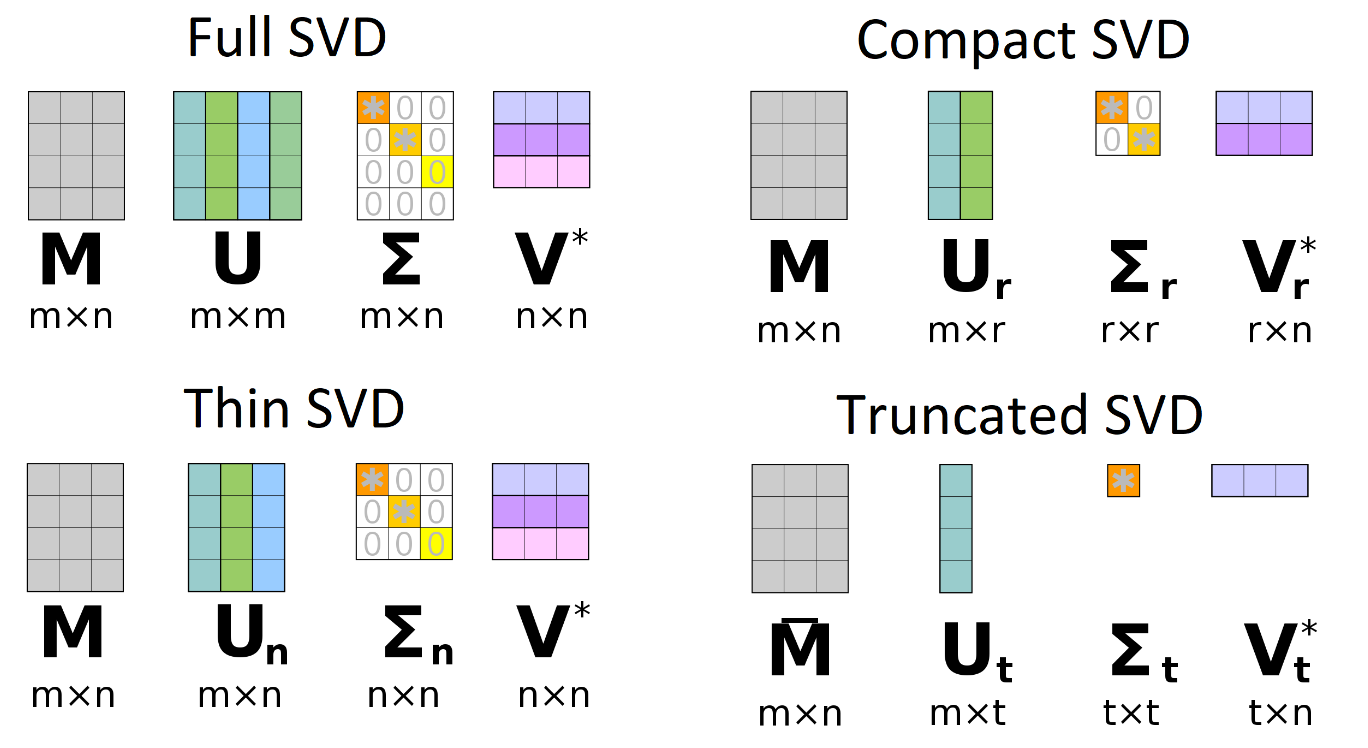
\includegraphics[width=\textwidth]{images/SVD.png}
  \caption{Confronto tra varianti della SVD.
  Full: $U\in\mathbb{R}^{m\times m}$, $\Sigma\in\mathbb{R}^{m\times n}$, $V^{\top}\in\mathbb{R}^{n\times n}$.
  Compact/Thin: $U_r\in\mathbb{R}^{m\times r}$, $\Sigma_r\in\mathbb{R}^{r\times r}$, $V_r^{\top}\in\mathbb{R}^{r\times n}$.
  Truncated: $U_t\in\mathbb{R}^{m\times t}$, $\Sigma_t\in\mathbb{R}^{t\times t}$, $V_t^{\top}\in\mathbb{R}^{t\times n}$ con $t<r$.}
  \label{fig:svd-variants}
\end{figure}

\subsection{Latent Semantic Analysis (LSA)}\label{subsec:lsa}
LSA applica la SVD alla matrice termine-documento (\S\ref{subsec:text2num}). Troncando ai primi $k$ valori singolari si ottiene uno spazio semantico di bassa dimensione che attenua sinonimia/rumore e migliora il recupero di informazione.

\section{Riduzione per trasformazione dei dati}\label{sec:riduzione-trasf}
Ridurre dimensionalità trasformando i dati in forme più compatte e \emph{strutturate}:
\begin{itemize}
  \item \textbf{Serie temporali}: trasformata di Fourier, trasformata wavelet di Haar.
  \item \textbf{Grafi}: embedding spettrali/\emph{multidimensional scaling} per preservare distanze/similarità tra nodi.
\end{itemize}
\chapter{Insiemi Frequenti e Regole d'Associazione}\label{ch:frequent-itemsets}
% Basato sulle slide del corso ("Mining insiemi frequenti -- Parte 1") e approfondimenti dal libro (Leskovec et al., cap. 6).

\section{Market-basket model e definizioni}\label{sec:mbm}
Nel \emph{market-basket model} ogni transazione (\emph{basket}) è un insieme di oggetti (\emph{item}). L'obiettivo è individuare \textbf{itemset frequenti}, cioè insiemi di item che compaiono assieme in molte transazioni, e derivarne \textbf{regole d'associazione} utili per descrivere co-occorrenze interessanti.

\paragraph{Supporto.} Sia $\mathcal{D}$ l'insieme dei basket (con $|\mathcal{D}|=N$) e sia $I=\{i_1,\dots,i_k\}$ un itemset. Il \textbf{supporto} assoluto di $I$ è
\[
\mathrm{supp}(I) = |\{ T\in\mathcal{D}\,:\, I\subseteq T\}|,\qquad \mathrm{supp}_\mathrm{rel}(I)=\frac{\mathrm{supp}(I)}{N}.
\]
Dato un valore soglia $\sigma$ (\emph{min-sup}), $I$ è detto \textbf{frequente} se $\mathrm{supp}(I)\ge \sigma$.

\paragraph{Soglia di supporto: trade-off.} Una soglia troppo alta può eliminare pattern interessanti; una troppo bassa produce un'esplosione di candidati difficili da analizzare e validare.

\section{Regole d'associazione}\label{sec:assoc}
Una \textbf{regola d'associazione} è un'implicazione $X\to j$, con $X$ itemset e $j$ un singolo item con $j\notin X$. Si estende naturalmente a $X\to Y$ con $X\cap Y=\varnothing$.

\subsection{Qualità di una regola}\label{subsec:qualita-regole}
\paragraph{Confidenza.} Con $\mathrm{supp}(\cdot)$ definito sopra, la confidenza di $X\to j$ è
\[
\mathrm{conf}(X\to j) = \frac{\mathrm{supp}(X\cup\{j\})}{\mathrm{supp}(X)} \;=\; P(j\mid X).\label{eq:confidence}
\]
\paragraph{Coverage.} $\mathrm{supp}(X)$ è detto anche \emph{coverage}: misura quanto spesso è applicabile la regola.
\paragraph{Interesse (o \emph{interest}).} Quantifica l'influenza di $X$ su $j$ come scostamento dalla prevalenza marginale di $j$:
\[
\mathrm{int}(X\to j) = \mathrm{conf}(X\to j) - \frac{\mathrm{supp}(\{j\})}{N}.
\]
\paragraph{Lift.} Confronta la co-occorrenza osservata con quella attesa in caso di indipendenza:
\[
\mathrm{lift}(X\to j) = \frac{N\cdot\mathrm{supp}(X\cup\{j\})}{\mathrm{supp}(X)\,\mathrm{supp}(\{j\})} \;=\; \frac{\mathrm{conf}(X\to j)}{\mathrm{supp}(\{j\})/N}.
\]
Valori $>1$ indicano associazione positiva, $<1$ negativa.

\paragraph{Nota.} Supporto e confidenza alti non implicano necessariamente interesse: regole ovvie (es. {pasta, pomodoro} $\to$ {pasta}) possono essere poco informative.

\subsection{Mini-esempio (dataset giocattolo)}\label{subsec:mini-esempio}
Sia $N=8$ e consideriamo item $\{b,c,j,m,p\}$. Supponiamo che $\mathrm{supp}(\{b\})=6$, $\mathrm{supp}(\{c\})=5$, $\mathrm{supp}(\{j\})=4$, $\mathrm{supp}(\{m\})=5$, $\mathrm{supp}(\{p\})=2$ e, tra le coppie, $\mathrm{supp}(\{b,c\})=4$, $\mathrm{supp}(\{c,j\})=3$, $\mathrm{supp}(\{c,m\})=2$, $\mathrm{supp}(\{m,p\})=2$, ecc. Per la regola $\{c,m\}\to b$ si ha
\[
\mathrm{conf}=\tfrac{\mathrm{supp}(\{b,c,m\})}{\mathrm{supp}(\{c,m\})}=\tfrac{2}{2}=1.0,\quad
\mathrm{lift}=\frac{8\cdot 2}{2\cdot 6}=1.33\,.
\]

\section{Insiemi frequenti chiusi e massimali}\label{sec:closed-maximal}
Sia $I$ frequente.
\begin{itemize}
  \item $I$ è \textbf{chiuso} se nessun suo super-insieme ha lo \emph{stesso} supporto di $I$.
  \item $I$ è \textbf{massimale} se nessun suo super-insieme è frequente.
\end{itemize}
Gli insiemi massimali sono (per definizione) chiusi; gli insiemi chiusi sono un sottoinsieme degli insiemi frequenti e consentono una rappresentazione più compatta senza perdere il supporto degli insiemi chiusi stessi.

\begin{figure}[htbp]
  \centering
  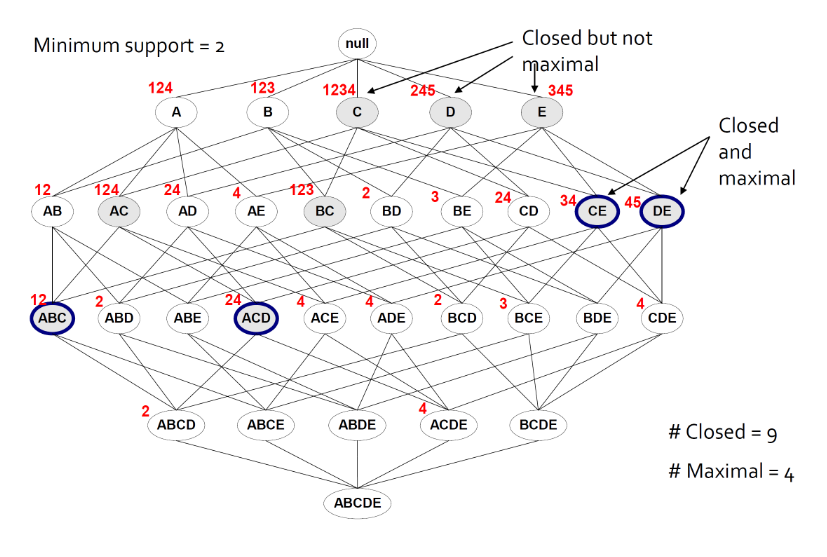
\includegraphics[width=0.8\textwidth]{images/insiemi_frequenti_massimale.png}
  \caption[Itemset lattice (minsup 2)]%
  {Grafo degli itemset con minsup $=2$. Un itemset è \emph{frequente} se il suo supporto è \texorpdfstring{$\ge 2$}{>= 2};
  è \emph{chiuso} se nessun superinsieme ha lo stesso supporto; è \emph{massimale} se nessun superinsieme è frequente.
  Nell'esempio: alcuni chiusi (es. CE) e chiusi–massimali (CE, DE); conteggi indicati: \#closed = 9, \#maximal = 4.}
  \label{fig:ifm}
\end{figure}


\section{Proprietà anti-monotona e Principio di Apriori}\label{sec:apriori-principle}
Per itemset $S\subseteq I$ vale l'\textbf{anti-monotonicità del supporto}:
\[
\mathrm{supp}(I)\le \mathrm{supp}(S).\label{eq:anti-mon}
\]
Da cui il \textbf{Principio di Apriori}: se un itemset $I$ è frequente, ogni suo sottoinsieme è frequente; equivalentemente, se $I$ non è frequente, nessun suo super-insieme può esserlo. Questa proprietà consente un \emph{pruning} efficace dello spazio dei candidati.

\section{Algoritmo Apriori}\label{sec:apriori}
Ricerca bottom-up per cardinalità crescente.
\begin{enumerate}
  \item Calcola l'insieme $L_1$ degli item singoli frequenti.
  \item Per $k=1,2,\dots$:
  \begin{enumerate}
    \item \textbf{Join}: genera $C_{k+1}$ (candidati di taglia $k{+}1$) con self-join di $L_k$.
    \item \textbf{Prune}: elimina da $C_{k+1}$ gli itemset che contengono sottoinsiemi di taglia $k$ non frequenti (per \S\ref{sec:apriori-principle}).
    \item \textbf{Conteggio}: calcola $\mathrm{supp}(\cdot)$ dei candidati scorrendo il DB e costruisci $L_{k+1}=\{c\in C_{k+1}: \mathrm{supp}(c)\ge\sigma\}$.
  \end{enumerate}
  \item Arresta quando $C_{k+1}=\varnothing$.
\end{enumerate}

\subsection{Apriori: esempio (minsup = 2)}\label{subsec:apriori-esempio}
Consideriamo $N=8$ basket e gli item $\{b,c,j,m,p\}$. I supporti degli item singoli sono:
\begin{center}
\begin{tabular}{@{}lccccc@{}}
\toprule
Item & $b$ & $c$ & $j$ & $m$ & $p$ \\
\midrule
$\mathrm{supp}(\cdot)$ & 6 & 5 & 4 & 5 & 2 \\
\bottomrule
\end{tabular}
\end{center}
Con minsup $=2$, tutti e cinque gli item sono frequenti, quindi $L_1=\{b,c,j,m,p\}$. \emph{(Dati come nelle slide)}.

\paragraph{Passo $k=1\to2$: generazione $C_2$ e pruning.}
$C_2$ si ottiene con self-join di $L_1$ e contiene tutte le coppie possibili:
\[
\{b,c\},\{b,j\},\{b,m\},\{b,p\},\{c,j\},\{c,m\},\{c,p\},\{j,m\},\{j,p\},\{m,p\}.
\]
Dai conteggi nel DB (come in tabella delle slide) si ottengono i supporti:
\begin{center}
\begin{tabular}{@{}lcccccccccc@{}}
\toprule
Itemset & $\{b,c\}$ & $\{b,j\}$ & $\{b,m\}$ & $\{b,p\}$ & $\{c,j\}$ & $\{c,m\}$ & $\{c,p\}$ & $\{j,m\}$ & $\{j,p\}$ & $\{m,p\}$ \\
\midrule
$\mathrm{supp}(\cdot)$ & 4 & 2 & 4 & 1 & 3 & 2 & 0 & 2 & 1 & 2 \\
\bottomrule
\end{tabular}
\end{center}
Applicando minsup, otteniamo $L_2=\{\{b,c\},\{b,j\},\{b,m\},\{c,j\},\{c,m\},\{j,m\},\{m,p\}\}$. 

\paragraph{Passo $k=2\to3$: generazione $C_3$ da $L_2$ (self-join) e pruning.}
Si combinano coppie con i primi $k-1$ item uguali (ordine lessicografico) e si rimuovono i candidati che hanno qualche sottoinsieme di taglia 2 non in $L_2$ (Principio di Apriori, \S\ref{sec:apriori-principle}). I candidati che restano sono:
\[
C_3=\{\{b,c,j\},\{b,c,m\},\{b,j,m\},\{c,j,m\}\}.
\]
Conteggiando i supporti sul DB (slide):
\begin{center}
\begin{tabular}{@{}lcccc@{}}
\toprule
Itemset & $\{b,c,j\}$ & $\{b,c,m\}$ & $\{b,j,m\}$ & $\{c,j,m\}$ \\
\midrule
$\mathrm{supp}(\cdot)$ & 2 & 2 & 1 & 1 \\
\bottomrule
\end{tabular}
\end{center}
Quindi $L_3=\{\{b,c,j\},\{b,c,m\}\}$.

\paragraph{Passo $k=3\to4$: generazione $C_4$ e arresto.}
L’unico candidato unibile è $\{b,c,j,m\}$, ma il suo supporto vale $1<2$, dunque non è frequente e $L_4=\varnothing$. L’algoritmo termina.

\paragraph{Riassunto dell’esempio.}
\[
L_1=\{b,c,j,m,p\},\quad
L_2=\{\{b,c\},\{b,j\},\{b,m\},\{c,j\},\{c,m\},\{j,m\},\{m,p\}\},
\]
\[
L_3=\{\{b,c,j\},\{b,c,m\}\},\quad
L_4=\varnothing.
\]
L’anti-monotonicità del supporto permette il \emph{pruning} efficace a ogni livello, riducendo drasticamente i candidati da contare. 


\subsection{Generazione dei candidati}\label{subsec:candidate-gen}
Se gli item sono ordinati, due insiemi $A=(a_1,\dots,a_{k-1},x)$ e $B=(a_1,\dots,a_{k-1},y)$ in $L_k$ con $x<y$ producono il candidato $(a_1,\dots,a_{k-1},x,y)$. Il passo di \emph{prune} scarta i candidati che hanno almeno un sottoinsieme di taglia $k$ non presente in $L_k$.

\paragraph{Esempio (schema).} Da $L_2=\{\{b,c\},\{b,j\},\{b,m\},\{c,j\},\{c,m\},\{j,m\},\{m,p\}\}$ si generano candidati di taglia 3 come $\{b,c,j\}$, $\{b,c,m\}$, $\{b,j,m\}$, $\{c,j,m\}$, ecc., poi si eliminano quelli che contengono coppie non frequenti.

\section{Ottimizzazioni di Apriori}\label{sec:apriori-opt}
\subsection{Hashing in bucket: PCY}\label{subsec:pcy}
Alla prima passata si contano i singoli item e, parallelamente, si proiettano tutte le coppie in bucket tramite una funzione hash. I bucket con supporto sotto soglia vengono marcati come non frequenti: alla seconda passata, una coppia $(i,j)$ è candidata solo se \emph{entrambi} gli item sono frequenti e il bucket hash di $(i,j)$ è frequente. Ciò riduce notevolmente $|C_2|$.

\subsection{Partizionamento del DB: SON}\label{subsec:son}
Divide il dataset in partizioni; su ciascuna partizione si esegue Apriori con min-sup scalato (proporzionale alla frazione di transazioni della partizione). L'unione degli insiemi frequenti locali fornisce i candidati globali, che vengono poi verificati su tutto il DB. L'algoritmo è adatto a calcolo distribuito.

\subsection{Campionamento e frontiera negativa: Toivonen}\label{subsec:toivonen}
Si esegue Apriori su un campione casuale $S$ con soglia più bassa ($\sigma'$); si ottiene un insieme di itemset frequenti in $S$ e la \emph{frontiera negativa}: insiemi non frequenti in $S$ i cui \emph{immediati} sottoinsiemi sono frequenti. Se nessun elemento della frontiera negativa risulta frequente sull'intero DB, i frequenti di $S$ sono la risposta; altrimenti si ripete con un nuovo campione (per evitare falsi negativi), regolando $\sigma'$.

\section{Perch\'e andare oltre Apriori}\label{sec:oltre-apriori}
Apriori richiede (i) generare esplicitamente i candidati $C_k$ a ogni livello e (ii) pi\`u passate sul database per calcolare i supporti. Con soglie basse o molti pattern, il numero di candidati esplode e le scansioni diventano costose. \textbf{FP-Growth} evita entrambi: rappresenta il DB in modo compatto (\emph{FP-tree}) e \emph{fa crescere} i pattern frequenti senza generare $C_k$.

\section{FP-Growth: idea di base}\label{sec:fpgrowth}
\begin{enumerate}
  \item \textbf{Costruzione FP-tree} (\emph{Frequent Pattern tree}): scansiona il DB per ottenere i supporti degli item, scarta quelli con supporto $<\sigma$, ordina gli item per supporto decrescente e inserisci le transazioni nell’albero condividendo i prefissi comuni. Mantieni una \emph{header table} con link ai nodi per item.
  \item \textbf{Pattern-growth}: per ogni item $x$ (dall’ultimo al primo nell’ordine per supporto) estrai la \emph{pattern base condizionale} di $x$ dai cammini che portano a $x$, costruisci l’\emph{FP-tree condizionale} e ripeti ricorsivamente. I pattern trovati si concatenano con $x$.
\end{enumerate}
Servono in genere \textbf{due passate} sul DB (una per i conteggi degli item, una per costruire l’albero); poi si lavora su strutture in memoria.

\subsection{Costruzione dell'FP-tree}\label{subsec:costruzione-fptree}
\begin{enumerate}
  \item \textbf{Prima passata}: calcola $\mathrm{supp}(i)$ per ogni item; elimina gli item con $\mathrm{supp}(i)<\sigma$.
  \item \textbf{Ordina} gli item per supporto decrescente (tie-break fisso) e \textbf{riordina} ogni transazione seguendo lo stesso ordine.
  \item \textbf{Inserisci} ciascuna transazione nell’albero a partire dalla radice: percorri/crea i nodi lungo il prefisso ordinato, incrementando i contatori dei nodi e aggiornando i \emph{node link} nella header table.
\end{enumerate}
\emph{Propriet\`a}: l’FP-tree conserva l’informazione necessaria a ricostruire i supporti dei pattern frequenti ed \`e molto compatto se molte transazioni condividono prefissi.

\subsection{Esempio di FP-Growth}\label{subsec:fpg-example}
Soglia $\sigma=3$. Dalla prima passata otteniamo gli item frequenti (con supporto) in ordine decrescente:
\[
f:4,\quad c:4,\quad a:3,\quad b:3,\quad m:3,\quad p:3.
\]
Ogni transazione viene \textbf{riordinata} secondo l’ordine $f\!\succ c\!\succ a\!\succ b\!\succ m\!\succ p$ ed \textbf{inserita} nell’FP-tree, aggregando i prefissi per incrementare i contatori.

\paragraph{Header table iniziale.}
\begin{center}
\begin{tabular}{@{}lcccccc@{}}
\toprule
Item & $f$ & $c$ & $a$ & $b$ & $m$ & $p$ \\
\midrule
$\mathrm{supp}(\cdot)$ & 4 & 4 & 3 & 3 & 3 & 3 \\
\bottomrule
\end{tabular}
\end{center}

\begin{figure}[htbp]
  \centering
  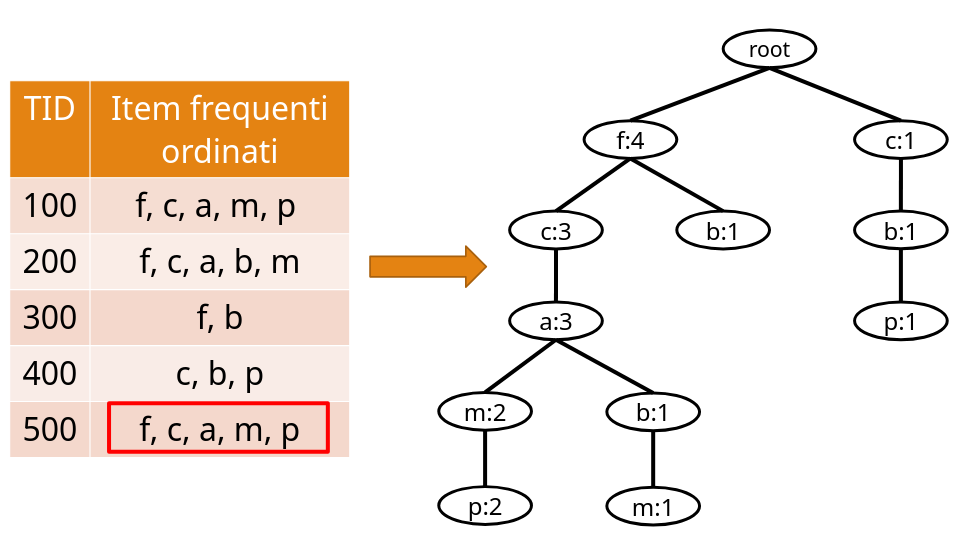
\includegraphics[width=0.92\textwidth]{images/fp-growth-complete.png}
  \caption{Costruzione dell’FP-tree: a sinistra le transazioni con gli item frequenti ordinati; a destra l’albero ottenuto condividendo i prefissi e incrementando i contatori dei nodi. L’ultima transazione (TID 500) segue il percorso f $\rightarrow$ c $\rightarrow$ a $\rightarrow$ m $\rightarrow$ p e aggiorna i relativi nodi.}
  \label{fig:fp-growth-complete}
\end{figure}

\paragraph{Visita per pattern-growth.}
Si processano gli item \emph{dal meno frequente al pi\`u frequente} nell’ordine della header table (a parit\`a, dall’ultimo al primo):
\[
p \rightarrow m \rightarrow b \rightarrow a \rightarrow c \rightarrow f.
\]

\paragraph{Come si espande un item $x$ (pattern-growth).}
\begin{enumerate}
  \item \textbf{Pattern base condizionale di $x$.} Segui i \emph{node link} di $x$ e,
        per ogni nodo $x$, prendi il cammino dalla radice al \emph{genitore} di $x$
        (escludi $x$). Assegna a quel cammino un \emph{peso} uguale al contatore del nodo $x$.
        % Multinsieme di cammini pesati: quali prefissi compaiono insieme a $x$ e quanto spesso.
  \item \textbf{FP-tree condizionale di $x$.} Dai cammini pesati:
        (i) somma i pesi per ogni item e \emph{rimuovi} quelli con supporto $<\sigma$;
        (ii) ordina gli item per supporto decrescente; 
        (iii) inserisci i cammini (con pesi) costruendo l’albero $T_x$.
  \item \textbf{Ricorsione e output.} I pattern frequenti che \emph{contengono} $x$
        sono $\{x\}$ unito a ciascun pattern frequente trovato in $T_x$.
        \emph{Caso speciale (cammino unico)}: se $T_x$ è una sola path,
        tutte le combinazioni dei suoi nodi sono frequenti; il supporto è il \emph{minimo} dei contatori lungo la combinazione.
\end{enumerate}

\begin{figure}[htbp]
  \centering
  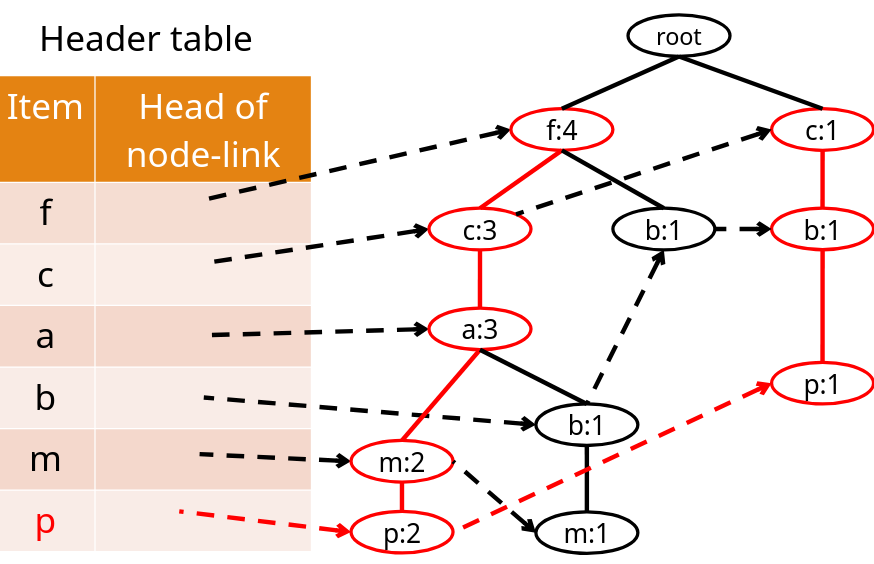
\includegraphics[width=0.9\textwidth]{images/fp-growth-links.png}
  \caption{Header table e node-link per l’item $p$: i puntini tratteggiati collegano le occorrenze di $p$ nell’FP-tree. Seguendo i node-link si raccolgono i cammini verso la radice (senza $p$) con i rispettivi contatori: questa è la pattern base condizionale di $p$, da cui si costruisce l’FP-tree condizionale $T_p$.}
  \label{fig:fp-growth-links}
\end{figure}

\paragraph{Esempio 1: item $p$.}
Supponiamo che, seguendo i \emph{node link} di $p$, si incontrino i cammini verso radice:
\[
\langle f,c,a,m\rangle:2 \quad \text{e} \quad \langle c,b\rangle:1.
\]
La \textbf{base condizionale} di $p$ \`e quindi $\{\langle f,c,a,m\rangle \text{ con peso } 2,\ \langle c,b\rangle \text{ con peso } 1\}$. Con $\sigma=3$ nessun sotto-pattern che include $p$ raggiunge la soglia (pesi massimi 2 e 1), dunque \emph{nessun} pattern frequente contiene $p$.

\paragraph{Esempio 2: item $m$.}
Cammini verso $m$ (esempio coerente con le slide):
\[
\langle f,c,a\rangle:2,\quad \langle f,c\rangle:1.
\]
La base condizionale di $m$ \`e $\{\langle f,c,a\rangle:2,\ \langle f,c\rangle:1\}$. Frequenze condizionali:
\[
\mathrm{supp}_{\mathrm{cond}}(f)=3,\ \mathrm{supp}_{\mathrm{cond}}(c)=3,\ \mathrm{supp}_{\mathrm{cond}}(a)=2.
\]
Con $\sigma=3$ risultano frequenti i pattern $\{m,f\}$, $\{m,c\}$ e, proseguendo, $\{m,f,c\}$ con supporto $3$ (intersezione dei cammini). 

\paragraph{Esempio 3: item $b$.}
Cammini verso $b$:
\[
\langle f,c,a\rangle:2,\quad \langle c\rangle:1.
\]
Base condizionale di $b$: $\{\langle f,c,a\rangle:2,\ \langle c\rangle:1\}$. Frequenze condizionali:
\[
\mathrm{supp}_{\mathrm{cond}}(c)=3,\ \mathrm{supp}_{\mathrm{cond}}(f)=2,\ \mathrm{supp}_{\mathrm{cond}}(a)=2.
\]
Con $\sigma=3$ si ottiene $\{b,c\}$ frequente; combinazioni con $f$ o $a$ non superano la soglia.

\section{Confronto: FP-Growth vs Apriori}\label{subsec:confronto-fp-apriori}
\begin{table}[htbp]
\centering
\begin{tabular}{@{}p{0.28\textwidth}p{0.33\textwidth}p{0.33\textwidth}@{}}
\toprule
\textbf{Aspetto} & \textbf{Apriori} & \textbf{FP-Growth} \\
\midrule
Generazione candidati &
Sì: crea $C_k$ a ogni livello (rischio di esplosione combinatoria) &
No: crescita diretta dei pattern dall’FP-tree \\
Accessi al DB &
Molte passate (una per ogni $k$) &
Tipicamente 2 passate, poi si lavora in memoria \\
Strutture dati principali &
Liste di candidati e conteggi &
FP-tree + header table (node-link) \\
Quando preferirlo &
DB piccoli/sparsi, soglie alte, ambienti distribuiti molto semplici &
DB densi, soglie basse, molti prefissi condivisi (compressione efficace) \\
Note pratiche &
Pruning con principio di Apriori, implementazione semplice &
Evita i candidati; molto veloce se l’FP-tree è compatto \\
\bottomrule
\end{tabular}
\caption{Confronto sintetico tra Apriori e FP-Growth.}
\label{tab:apriori-vs-fpgrowth}
\end{table}
\chapter{Clustering}\label{ch:clustering}

\section{Concetti generali}\label{sec:clu-concetti}
Il \textbf{clustering} raggruppa oggetti in \emph{cluster} tali che i punti nello stesso cluster siano tra loro simili, mentre punti in cluster diversi siano dissimili. È un compito \emph{unsupervised}: non si conoscono etichette a priori. La \emph{classificazione} è invece \emph{supervised} e richiede classi note per l’addestramento.

\subsection{Spazi metrici e funzioni distanza}\label{subsec:metric-spaces}
Si assume uno \textbf{spazio metrico} $(\mathcal{S},D)$, con $D$ che soddisfa:
\[
\begin{aligned}
\text{\textbf{Non negatività}}\quad & D(x,y) \ge \,0 && \forall\, x,y \in S,\\
\text{\textbf{Simmetria}}\quad & D(x,y) = D(y,x) && \forall\, x,y \in S,\\
\text{\textbf{Disuguaglianza triangolare}}\quad & D(x,y)+D(y,z) \ge D(x,z) && \forall\, x,y,z \in S.
\end{aligned}
\]

\paragraph{Distanze in spazi euclidei.}
Siano $\mathbf{x}=(x_1,\dots,x_n)$ e $\mathbf{y}=(y_1,\dots,y_n)\in\mathbb{R}^n$.

\[
\textbf{Distanza euclidea:}\quad
D_2(\mathbf{x},\mathbf{y})=\sqrt{\sum_{i=1}^{n}(x_i-y_i)^2}
\]

\[
\textbf{Distanza di Manhattan:}\quad
D_1(\mathbf{x},\mathbf{y})=\sum_{i=1}^{n}\lvert x_i-y_i\rvert
\]

\[
\textbf{Norma }L_r:\quad
D_r(\mathbf{x},\mathbf{y})=\Bigg(\sum_{i=1}^{n}\lvert x_i-y_i\rvert^{\,r}\Bigg)^{\!1/r},\ \ r\ge 1
\]

\[
\textbf{Norma }L_{\infty}:\quad
D_{\infty}(\mathbf{x},\mathbf{y})=\max_{1\le i\le n}\lvert x_i-y_i\rvert
\]

\[
\textbf{Distanza del coseno (angolare):}\quad
D_{\angle}(\mathbf{x},\mathbf{y})
=\arccos\!\left(
\frac{\sum_{i=1}^{n} x_i y_i}{\sqrt{\sum_{i=1}^{n} x_i^{2}}\ \sqrt{\sum_{i=1}^{n} y_i^{2}}}
\right),
\qquad \mathbf{x}\neq\mathbf{0},\ \mathbf{y}\neq\mathbf{0}.
\]



\paragraph{Spazi non euclidei.}
Per oggetti-insiemi o stringhe il centroide può non avere senso: si usa il \textbf{medoide} (elemento del dataset che minimizza la somma delle distanze agli altri).
Esempi di metriche:
\[
D_\mathrm{Jac}(S,T)=1- \frac{|S\cap T|}{|S\cup T|}\quad\text{(Jaccard)},
\]
Altri esempi di distanze sono:
\begin{enumerate}
  \item \textbf{Distanza di Edit}: il minimo numero di operazioni di cancellazione o inserzioni di caratteri da effettuare partendo da una stringa A per ottenere la stringa B. (es. A = abcde, B = acfdeg $\Rightarrow$ D(A, B) = 3).
  \item \textbf{Distanza di Hamming}: dati A, B vettori, il numero di componeneti in corrispondenza delle quali differiscono (es. A = (1, 0, 1, 0, 1), B = (1, 1, 1, 1, 0) $\Rightarrow$ D(A, B) = 3).
\end{enumerate}

\subsection{Tassonomia degli algoritmi}\label{subsec:taxonomy}
Tre famiglie principali:

\begin{enumerate}
  \item \textbf{gerarchici} (agglomerativi/divisivi);
  \item \textbf{partizionali} (es.\ k-means);
  \item \textbf{a densità} (DBSCAN/OPTICS/HDBSCAN).
\end{enumerate}

\paragraph{Bontà di un algoritmo.}
Dipende da: \emph{scalabilità}, supporto a attributi eterogenei, capacità di cogliere \emph{forme diverse} di cluster, \emph{robustezza} a outlier/rumore e dati mancanti, \emph{stabilità} all’aggiunta di nuovi dati, e \emph{interpretabilità} dei risultati. La scelta pratica è un compromesso tra qualità e costi computazionali.

\subsection{Alta dimensionalità: equidistanza e ortogonalità}\label{subsec:curse}
Spazi euclidei ad elevata dimensionalità soffrono del \emph{problema della dimensionalità}:
\begin{itemize}
  \item quasi tutte le coppie di punti risultano \textbf{equidistanti} e lontane tra loro;
  \item quasi tutte le coppie di vettori sono quasi \textbf{ortogonali}.
\end{itemize}

\paragraph{Equidistanza dei punti.}
Sia $D(\mathbf{x},\mathbf{y})=\|\mathbf{x}-\mathbf{y}\|_2$ con $\mathbf{x},\mathbf{y}\in[0,1]^n$ indipendenti.
Quando $n$ è grande, con alta probabilità:
\[
\underbrace{1}_{\text{limite inferiore}} \ \lesssim\ D(\mathbf{x},\mathbf{y})\ \lesssim\ \underbrace{\sqrt{n}}_{\text{limite superiore}}
\]
e \emph{solo una frazione trascurabile} di coppie è vicina ai due limiti. La \textbf{maggior parte} delle coppie ha una distanza
vicina alla media, circa $\sqrt{n}/3$ (concentrazione della distanza). Inoltre i prodotti scalari tendono a $0$,
così gli angoli sono prossimi a $90^\circ$ (quasi ortogonalità).

\paragraph{Conseguenze pratiche.}
Distinguerre “vicini” da “lontani” diventa difficile; conviene standardizzare le feature, ridurre la dimensionalità (es.\ PCA)
o usare metriche più adatte (cosine/angolare), soprattutto in presenza di dati sparsi.


\section{Clustering gerarchico}\label{sec:hierarchical}
\paragraph{Schema agglomerativo.}
(a) inizializza: ogni punto è un cluster; (b) ripeti: fonde i due cluster più vicini secondo una \emph{distanza tra cluster}; (c) termina con un criterio (numero desiderato di cluster o qualità).

\subsection{Distanza tra cluster (\emph{linkage})}\label{subsec:linkages}

\begin{figure}[htbp]
\centering
\begin{minipage}[t]{0.65\textwidth}
\vspace{0pt}
\begin{itemize}[leftmargin=1.2em]
  \item \textbf{Single-link}: $\min\{D(x,y): x\in C_i,\ y\in C_j\}$ (tende a catene).
  \item \textbf{Complete-link}: $\max\{D(x,y): x\in C_i,\ y\in C_j\}$ (favorisce cluster compatti).
  \item \textbf{Average-link}: media delle distanze su tutte le coppie $x\in C_i,\,y\in C_j$ (compromesso).
  \item \textbf{Centroid/medoid}: distanza tra centroidi (euclideo) o tra medoidi (generale).
\end{itemize}
\end{minipage}\hfill
\begin{minipage}[t]{0.27\textwidth}
\vspace{0pt}
\centering
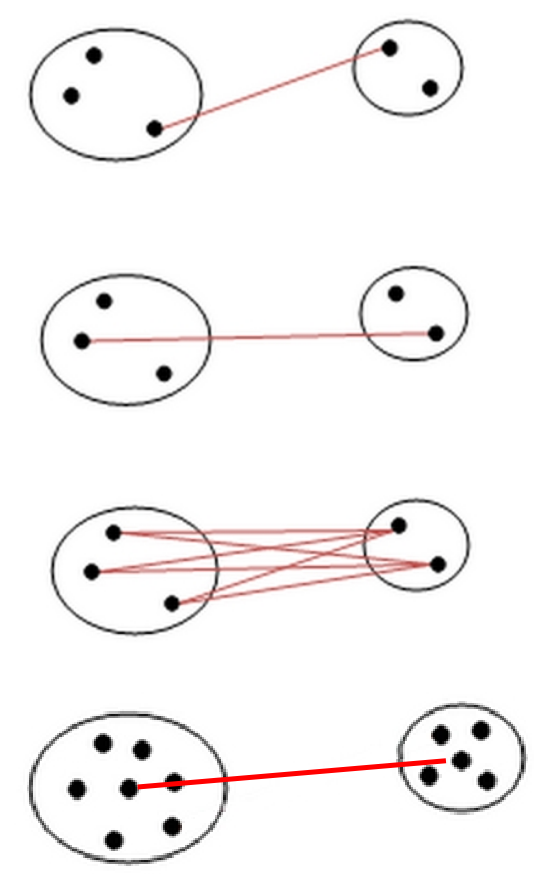
\includegraphics[width=\linewidth]{images/cluster_distances.png}
\caption{Esempi grafici delle diverse nozioni di distanza tra cluster.}
\label{fig:cluster_distances}
\end{minipage}
\end{figure}

\subsection{Dendrogramma e criteri di stop}\label{subsec:dendro}
Il \textbf{dendrogramma} registra le fusioni; tagliandolo a una certa altezza si ottiene la partizione.
Criteri di terminazione:
(i) fermarsi a $k$ cluster prefissati;
(ii) fermarsi quando l’unione successiva degrada troppo la qualità (es.\ aumento del diametro o della distanza media intra-cluster).

\begin{figure}
  \centering
  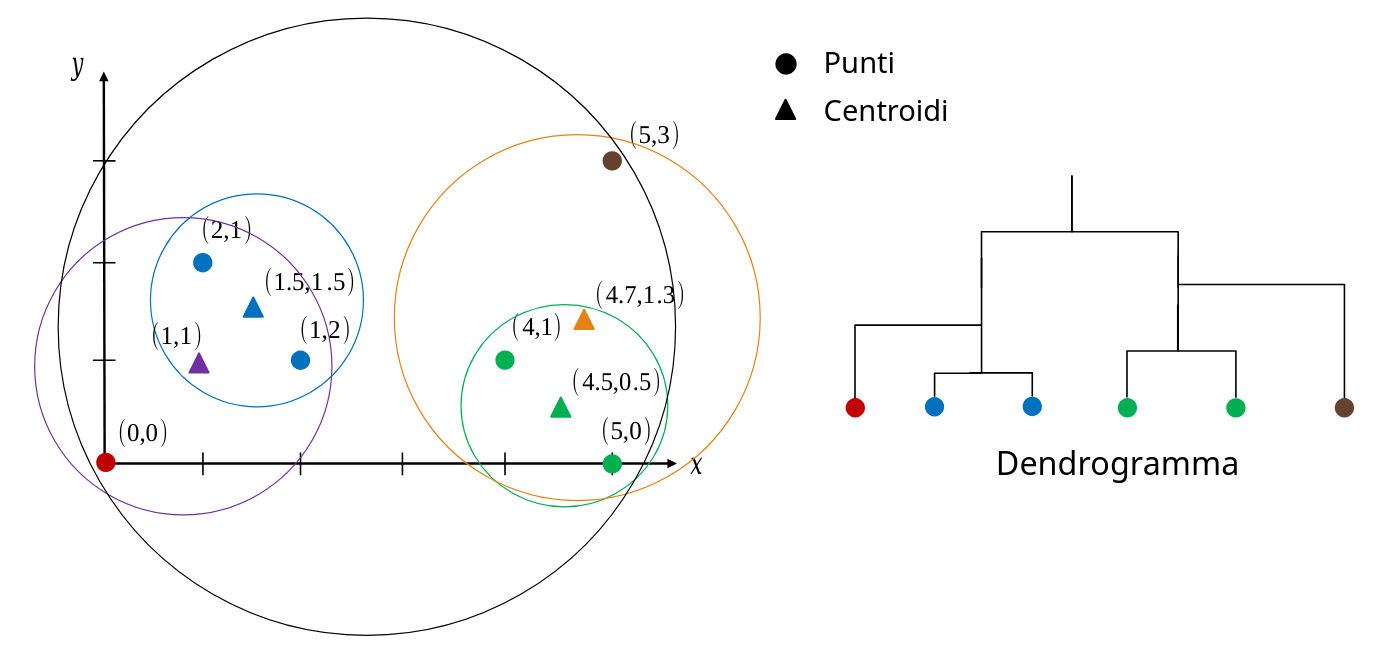
\includegraphics[width=\textwidth]{images/dendograms.png}
  \caption{A sinistra: punti nel piano con centroidi (triangoli) e cerchi che schematizzano la coesione dei gruppi; i colori indicano i cluster. A destra: dendrogramma agglomerativo che mostra l’ordine di fusione e l’altezza (distanza di linkage). Un taglio orizzontale del dendrogramma determina il numero di cluster.}
  \label{fig:dendograms}
\end{figure}

\subsection{Altri criteri di combinazione}\label{subsec:altri-criteri}
Si può fondere la coppia che massimizza la \emph{qualità} del cluster risultante.
Definizioni utili: \emph{raggio} $=\max_{x\in C} D(x,\mathrm{centroide}(C))$; \emph{diametro} $=\max_{x,y\in C} D(x,y)$.

\subsection{Versioni divisive}\label{subsec:divisive}
Approccio \textbf{top–down}: un'altra versione dove si parte da un unico cluster e lo si \emph{divide} iterativamente scegliendo il miglior \emph{taglio}. Le stesse metriche di distanza/qualità si applicano in modo duale.

\subsection{Complessità e ottimizzazioni}\label{subsec:hclust-compl}

\paragraph{Analisi \emph{naive}.}
Al primo passo si valuta la distanza per ogni coppia di cluster e si sceglie la migliore: costo $\Theta(n^2)$.
Dopo ogni fusione i cluster diminuiscono di uno, quindi i passi successivi costano, nell’ordine,
$(n-1)^2,(n-2)^2,\dots,2^2$.
\[
T_{\text{naive}}
=\sum_{k=2}^{n} k^{2}
=\frac{n(n+1)(2n+1)}{6}-1
=\Theta(n^{3}).
\]
(Spazio tipico: matrice delle distanze $O(n^2)$.)

\paragraph{Ottimizzazione con \emph{coda di priorità}.}
Usando una coda di priorità (min-heap) sulle distanze tra cluster:
\begin{itemize}
  \item accesso al minimo (\emph{peek}) in $O(1)$; inserimenti e cancellazioni in $O(\log n)$;
  \item ad ogni fusione si \emph{rimuovono} al più $2(n-1)$ distanze (quelle dai due cluster che si fondono): $O(n\log n)$;
  \item si \emph{calcolano e inseriscono} le distanze tra il nuovo cluster e gli altri (al più $n-2$): $O(n\log n)$.
\end{itemize}
Su $n-1$ fusioni:
\[
T_{\text{heap}}=O\big(n \cdot (n\log n)\big)=O(n^{2}\log n).
\]
Risultato: la complessità scende da $O(n^{3})$ a circa $O(n^{2}\log n)$ mantenendo la matrice (o la coda) aggiornata a ogni iterazione.


\section{Clustering partizionale: k-means}\label{sec:kmeans}
Metodi per spazi euclidei che partizionano i dati in $k$ cluster minimizzando la somma delle distanze al quadrato dai centroidi.

\subsection{Algoritmo base}\label{subsec:kmeans-basic}
\begin{enumerate}
  \item \textbf{Inizializza} $k$ centroidi (idealmente separati).
  \item \textbf{Assegna} ogni punto al centroide più vicino (distanza euclidea).
  \item \textbf{Aggiorna} ogni centroide come media dei punti assegnati.
  \item \textbf{Ripeti} finché i centroidi si stabilizzano o il miglioramento è sotto soglia.
\end{enumerate}
Converge in pochi round, ma solo a un ottimo \emph{locale}.

\subsection{Inizializzazione}\label{subsec:init}
Scelta \emph{greedy}:
\begin{enumerate}
  \item Si sceglie il primo punto in maniera casuale o lo si aggiunge all'insieme $S$ dei punti già selezionati, inizialmente vuoto.
  \item Si calcola la massima distanza minima dai centroidi scelti.
  \item Si ripete il passo 2. finché $|s| < k$.
\end{enumerate}

\begin{figure}[htpb]
  \centering
  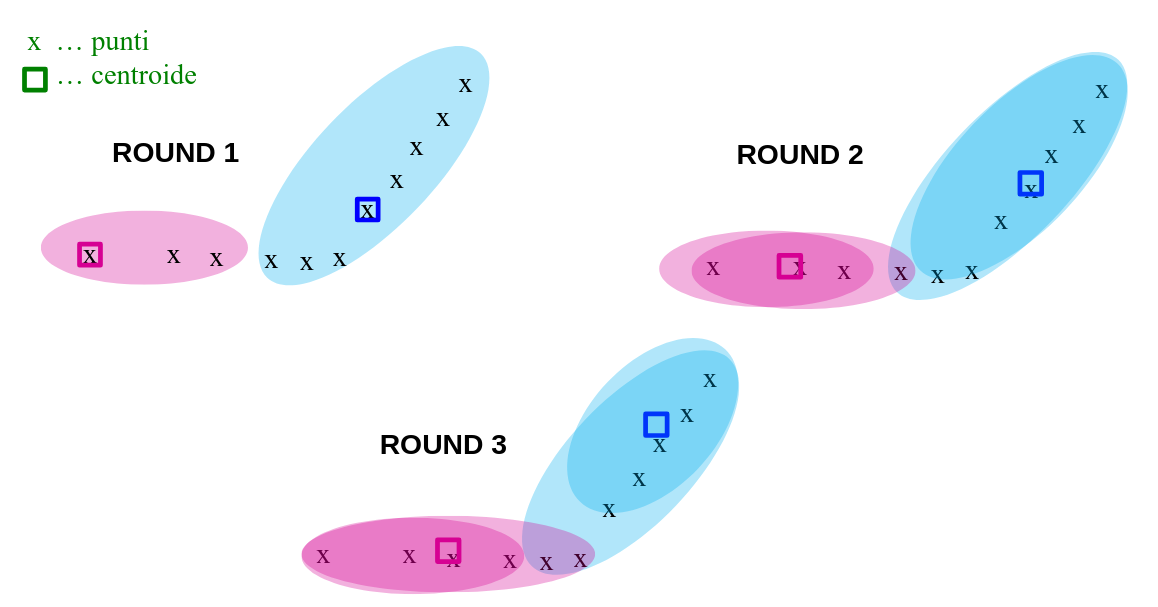
\includegraphics[width=0.7\textwidth]{images/k-means.png}
  \caption{K-means: evoluzione in tre round. 
  Round 1: inizializzazione e prime assegnazioni ai centroidi (quadrati). 
  Round 2: ricalcolo dei centroidi e riassegnazione dei punti (X). 
  Round 3: i centroidi si stabilizzano e i cluster (ellissi colorate) convergono.}
  \label{fig:k-means-example}
\end{figure}

\subsection{Funzione obiettivo e arresto}\label{subsec:objective}
Con partizione $C_1,\dots,C_k$ e centroidi $\mu_r$:
\[
J=\sum_{r=1}^k \sum_{x\in C_r} \|\mathbf{x}-\mu_r\|_2^2.
\]
Arresto quando $\Delta J$ tra iterazioni consecutive è sotto soglia o quando non cambia l’assegnazione. Con metriche diverse da euclidea il centroide non è il minimizzatore naturale.

\subsection{Scelta del numero di cluster $k$}\label{subsec:scelta-k}
Poiché $k$ non è noto a priori, si esegue il metodo per più valori e si seleziona quello che ottimizza una metrica di qualità interna.

\paragraph{Funzione obiettivo.}
Per $k$ cluster $C_1,\dots,C_k$ con centroidi $\mathbf{c}_1,\dots,\mathbf{c}_k$, la funzione standard è
\[
W(k)=\sum_{i=1}^k \sum_{\mathbf{x}\in C_i}\|\mathbf{x}-\mathbf{c}_i\|_2^2,\qquad 
\bar W(k)=\frac{W(k)}{n}\;\;(\text{distanza media al centroide}).
\]
$W(k)$ è decrescente in $k$.

\begin{figure}[htbp]
  \centering
  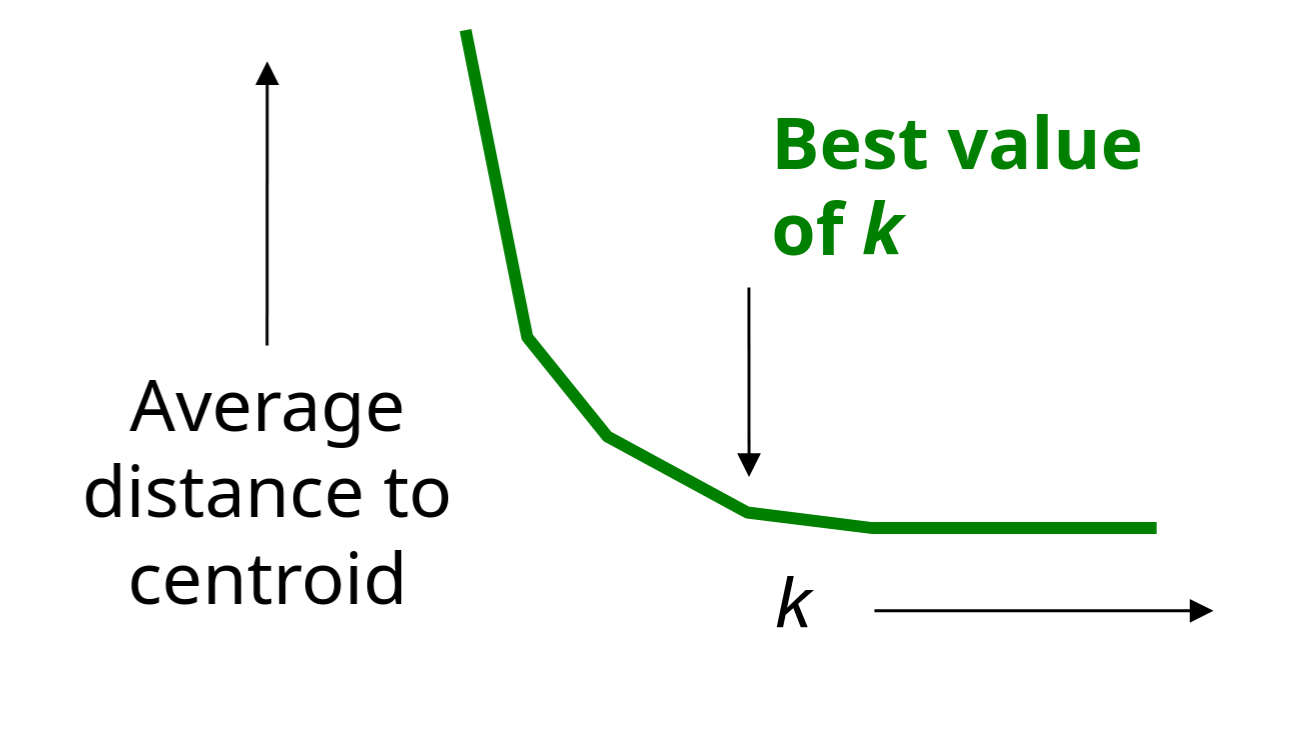
\includegraphics[width=0.8\textwidth]{images/elbow-k.png}
  \caption{Metodo (\emph{elbow}). Si traccia la distanza media dal centroide (o WCSS/n) al variare di $k$; il valore “ottimo” è nel punto di flesso, dove l’aumento di $k$ porta benefici marginali trascurabili.}
  \label{fig:elbow}
\end{figure}

\paragraph{Metodo \emph{elbow}.}
Si calcola $\bar W(k)$ per $k=k_{\min},\dots,k_{\max}$ e si sceglie il $k$ per cui il calo di $\bar W$ passa da “ripido” a “lento” (punto di flesso).
\begin{itemize}
  \item \emph{Procedura pratica:} si valuta $\bar W(k)$ su una griglia di valori e si ispeziona il grafico $\bar W$ vs $k$.
  \item \emph{Variante a ricerca binaria:} fissati due estremi $x<y$, si prende $z=\lfloor(x+y)/2\rfloor$, si calcola $\bar W(z)$ e si sostituisce l’estremo \emph{più vicino} a $\bar W(z)$ con $z$; si ripete finché l’intervallo è piccolo. Il $k$ finale approssima il gomito.
\end{itemize}
\emph{Nota:} se la curva non mostra un gomito netto, l’elbow diventa ambiguo e conviene affiancarlo a silhouette/stabilità.



\paragraph{Metodo \emph{silhouette}.}
Per ogni punto $\mathbf{x}$ assegnato al cluster $C_i$:
\[
a(\mathbf{x})=\frac{1}{|C_i|-1}\sum_{\mathbf{y}\in C_i,\ \mathbf{y}\neq \mathbf{x}}\!\!\!\!\|\mathbf{x}-\mathbf{y}\|, \qquad
b(\mathbf{x})=\min_{j\neq i}\ \frac{1}{|C_j|}\sum_{\mathbf{y}\in C_j}\|\mathbf{x}-\mathbf{y}\|.
\]
Lo \emph{score di silhouette} del punto è
\[
s(\mathbf{x})=\frac{b(\mathbf{x})-a(\mathbf{x})}{\max\{a(\mathbf{x}),\,b(\mathbf{x})\}}\in[-1,1].
\]
Valori vicini a $1$ indicano assegnazioni “pulite”, vicini a $0$ punti al confine, negativi assegnazioni sbagliate. Si sceglie
\[
k^\star=\arg\max_k\ \frac{1}{n}\sum_{r=1}^n s(\mathbf{x}_r).
\]
\emph{Regole d’uso.} Calcolare gli indici su più esecuzioni (inizializzazioni diverse) e riportare media/deviazione; standardizzare le feature prima del confronto; evitare $k$ troppo grandi che trivialiscono $\bar W$ ma peggiorano la silhouette.

% --------------------------------------------------------------------

\subsection{Complessità computazionale}\label{subsec:kmeans-compl}
Ogni iterazione del \emph{k}-means ha due passi:
\begin{enumerate}
  \item \textbf{Assegnamento} (nearest–centroid): per ciascun punto si valuta la distanza verso i $k$ centroidi. Costo $O(nkd)$ in $\mathbb{R}^d$ (spesso si sottintende $d$, scrivendo $O(nk)$).
  \item \textbf{Aggiornamento dei centroidi}: si ricalcolano le medie dei cluster. Costo $O(nd)$.
\end{enumerate}
Con $t$ iterazioni totali:
\[
T(n,k,d,t)=O(t\,n\,k\,d)\quad\text{(nelle slide: }O(tkn)\text{)}.
\]

\chapter{Classificazione}\label{ch:classificazione}

\section{Introduzione}\label{sec:intro-class}
La \textbf{classificazione} suddivide un insieme di dati in \emph{classi} note a priori (etichette),
apprendendo da esempi etichettati come assegnare la classe a nuove tuple. È quindi
\emph{apprendimento supervisionato}. Al contrario, il \emph{clustering} non parte da etichette
(\emph{unsupervised}) e scopre gruppi per similarità.

\paragraph{Predizione (regressione).}
Quando il target è \emph{numerico continuo}, il compito è di \emph{predire} un valore reale
(apprendimento supervisionato \emph{continuo}), cercando una funzione che approssimi
il target, non un confine tra classi.

\subsection{Schema generale di un classificatore}\label{subsec:schema-class}
\begin{enumerate}
  \item \textbf{Costruzione del modello} (training): si apprende da un \emph{training set} etichettato.
  \item \textbf{Validazione/valutazione} (test): si misura la bontà su un \emph{test set} etichettato.
  \item \textbf{Uso} (deploy): si applica il modello a nuove tuple per predirne la classe.
\end{enumerate}

\paragraph{Overfitting.}
L’overfitting si verifica quando un modello “impara a memoria” il training, compreso il rumore: va molto bene sui dati visti ma generalizza male su dati nuovi. In pratica è un segnale che il modello è troppo complesso rispetto alle informazioni disponibili. Per ridurlo, si separano chiaramente i dati per la verifica e si preferiscono soluzioni più semplici quando offrono prestazioni simili.

\begin{figure}[htbp]
  \centering
  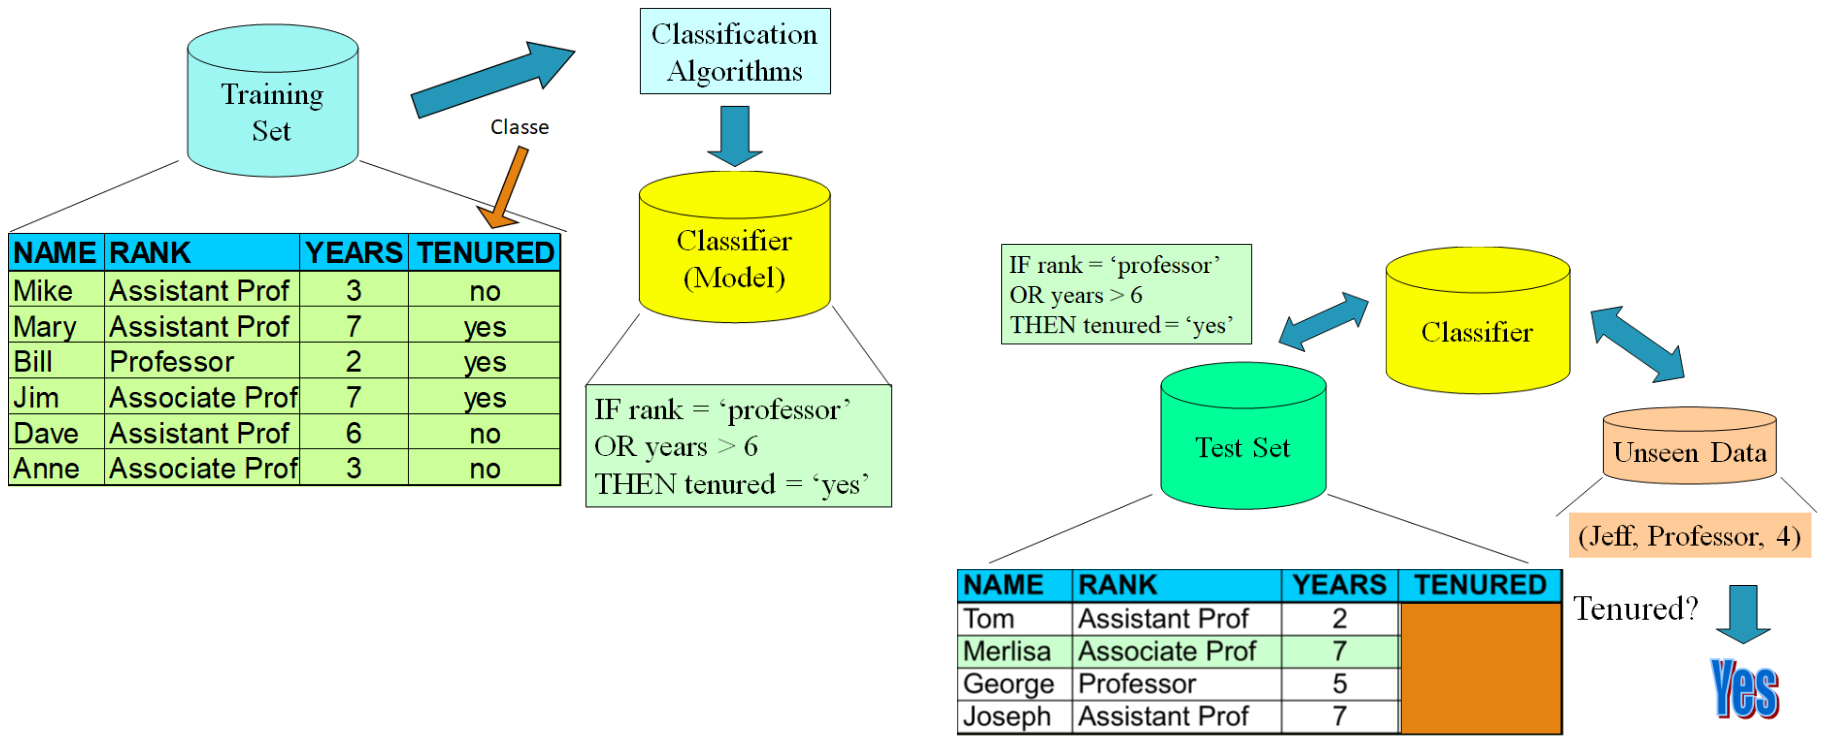
\includegraphics[width=.72\textwidth]{images/schema_classificatore.png}
  \caption{Schema a blocchi di un classificatore: addestramento, validazione e uso.}
  \label{fig:schema-class}
\end{figure}

\subsection{Requisiti desiderabili}\label{subsec:req}
\begin{itemize}
  \item \textbf{Accuratezza}: corretta predizione delle classi (o del valore, per i predittori).
  \item \textbf{Velocità}: tempi di training e di classificazione contenuti.
  \item \textbf{Robustezza}: tolleranza a rumore e dati mancanti.
  \item \textbf{Scalabilità}: efficienza su dataset di grandi dimensioni.
\end{itemize}

% ==========================================================
\section{Alberi decisionali}\label{sec:trees}
Gli \textbf{alberi decisionali} classificano applicando test su attributi lungo i nodi interni;
le \emph{foglie} portano le etichette di classe.

\subsection{Classificazione tramite albero}\label{subsec:tree-class}
La classe di una tupla $q$ si ottiene seguendo il cammino radice$\to$foglia guidato
dai test. Ogni cammino implementa una regola \texttt{IF-THEN} (le condizioni interne sono congiunte in AND). L’insieme di regole è \emph{esaustivo} e \emph{mutuamente esclusivo} (ogni tupla è coperta da una sola regola).

\begin{figure}[htbp]
  \centering
  \begin{minipage}[t]{.50\textwidth}
    \centering
    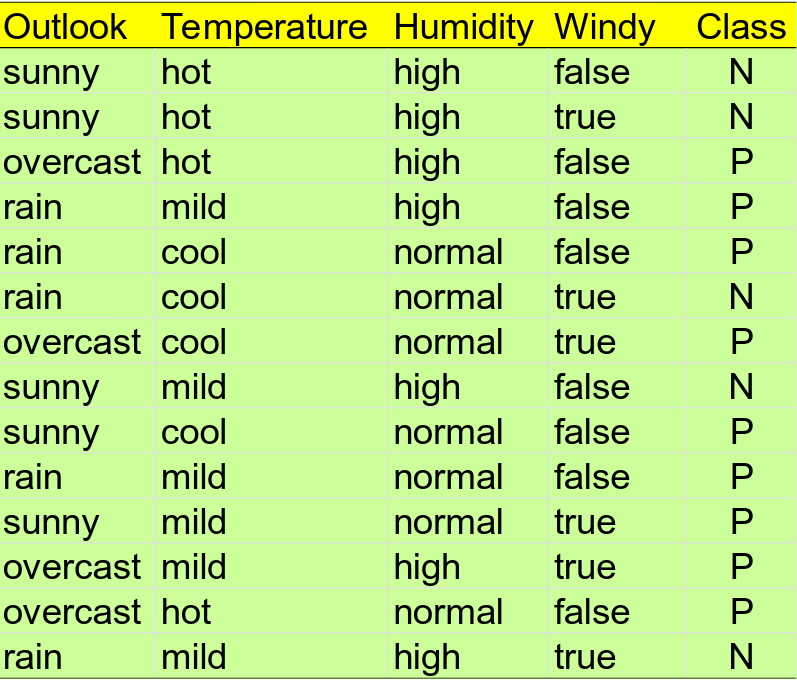
\includegraphics[width=\linewidth]{images/weather_table.png}
  \end{minipage}\hfill
  \begin{minipage}[t]{.48\textwidth}
    \centering
    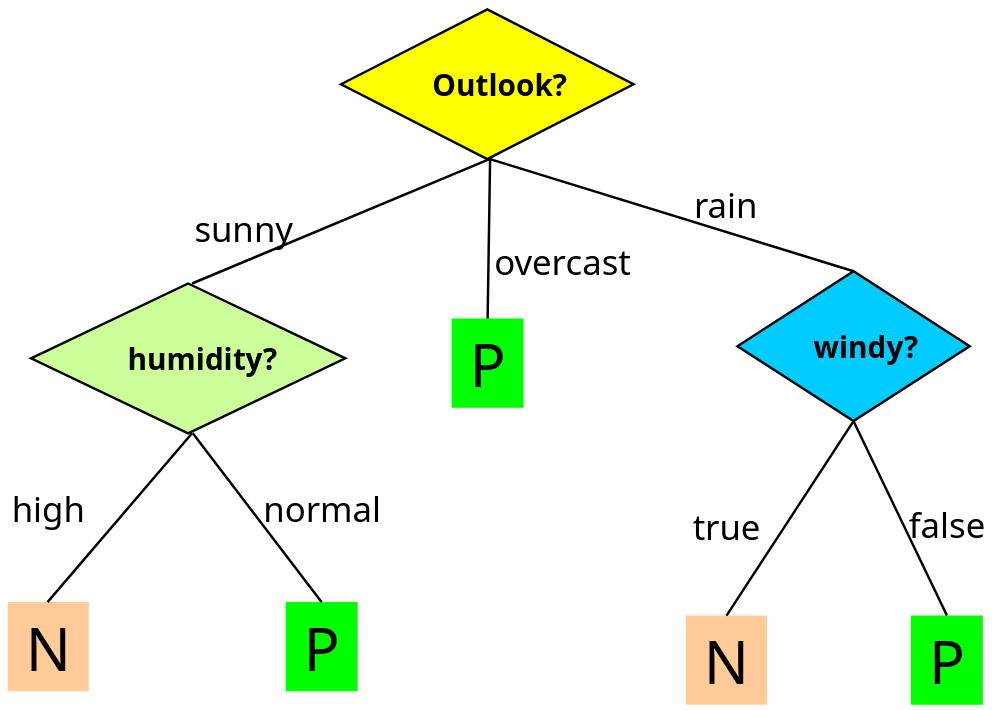
\includegraphics[width=\linewidth]{images/decision_tree_weather.png}
  \end{minipage}
  \caption{Dataset \emph{weather} (a sinistra) e albero decisionale appreso (a destra). 
  La tabella contiene 14 esempi con quattro attributi descrittivi (\texttt{Outlook}, \texttt{Temperature}, 
  \texttt{Humidity}, \texttt{Windy}) e la classe binaria \texttt{P/N}. 
  L’albero (stile ID3/C4.5) sceglie come radice \texttt{Outlook}; il ramo \texttt{overcast} porta 
  direttamente alla classe \texttt{P}, mentre per \texttt{sunny} si testa \texttt{Humidity} e per \texttt{rain} 
  si testa \texttt{Windy}. L’esempio illustra il passaggio da dati tabellari a regole interpretabili.}
  \label{fig:weather-tree}
\end{figure}


\newpage
\subsection{Costruzione top–down}\label{subsec:topdown}
Costruzione ricorsiva dalla radice:
\begin{enumerate}
  \item Se tutte le tuple del nodo $X$ hanno la \emph{stessa} classe $C$, crea una foglia $C$.
  \item Altrimenti scegli un attributo $A$ (non ancora usato) e \emph{ramifica} $X$ (\emph{splitting}) secondo i valori/soglia di $A$; crea i figli.
  \item Per ogni figlio $X_i$: se puro, fermati; se impuro, ripeti ricorsivamente.
\end{enumerate}

\paragraph{Pruning.}
Se le tuple nel nodo sono poche o la profondità è elevata, si può fermare prima e rendere il nodo una foglia (classe di maggioranza, oppure distribuzione di classe).

\subsection{Splitting degli attributi}\label{subsec:splitting}
\begin{itemize}
  \item \textbf{Booleani/numerici}: split \emph{binario} su soglia $t$ (``$\le t$'' a sinistra, ``$>t$'' a destra).
  \item \textbf{Categoriali}: split \emph{binario} definendo un sottoinsieme non vuoto di valori (a sinistra se il valore \emph{non} appartiene al sottoinsieme, a destra altrimenti).
\end{itemize}

\subsection{Scelta dell’attributo e strategia greedy}\label{subsec:greedy}
L’albero minimale è un problema \emph{NP-hard}; si usa una strategia \emph{greedy} che, ad ogni passo, seleziona l’attributo con massima \emph{goodness} (partizioni più pure),
costruendo l’albero “più compatto” possibile.

\subsection{Misure di goodness: Information Gain (ID3)}\label{subsec:ig}
Sia $S_X$ l’insieme di tuple al nodo $X$, con due classi $P$ e $N$; si indichino con $p$
e $n$ le rispettive numerosità. L’\textbf{entropia} di $S_X$ è
\[
H(S_X)\;=\; -\frac{p}{p+n}\log_2\!\frac{p}{p+n}\;-\;\frac{n}{p+n}\log_2\!\frac{n}{p+n}.
\]
Sia $A$ un attributo con $k$ valori distinti, che induce la partizione
$S_X \to S_1,\dots,S_k$. Se $S_i$ contiene $p_i$ e $n_i$ elementi, allora
\[
H(S_i)\;=\; -\frac{p_i}{|S_i|}\log_2\!\frac{p_i}{|S_i|}\;-\;\frac{n_i}{|S_i|}\log_2\!\frac{n_i}{|S_i|},\qquad
\overline{H}_A(S_X)\;=\;\sum_{i=1}^k \frac{|S_i|}{|S_X|}\,H(S_i).
\]
L’\textbf{information gain} dello split su $A$ è
\[
\mathrm{Gain}(S_X,A)\;=\;H(S_X)\;-\;\overline{H}_A(S_X).
\]
Si sceglie l’attributo con gain massimo.

\subsection{Esempio e limitazioni}\label{subsec:ig-example}
Sul dataset “weather” (Fig.~\ref{fig:weather-tree}) si ottengono:
\[
\mathrm{Gain}(\textit{outlook})=0.246,\quad
\mathrm{Gain}(\textit{temperature})=0.029,\quad
\mathrm{Gain}(\textit{humidity})=0.151,\quad
\mathrm{Gain}(\textit{windy})=0.048.
\]
\noindent
\textbf{Limite noto.} L’Information Gain è \emph{sbilanciato} verso attributi con molti valori:
un attributo quasi univoco (es.\ \texttt{ID}) produce molte partizioni piccole (foglie pure),
abbattendo l’entropia media e gonfiando artificialmente il gain, pur senza reale capacità
predittiva.

\begin{figure}[htbp]
  \centering
  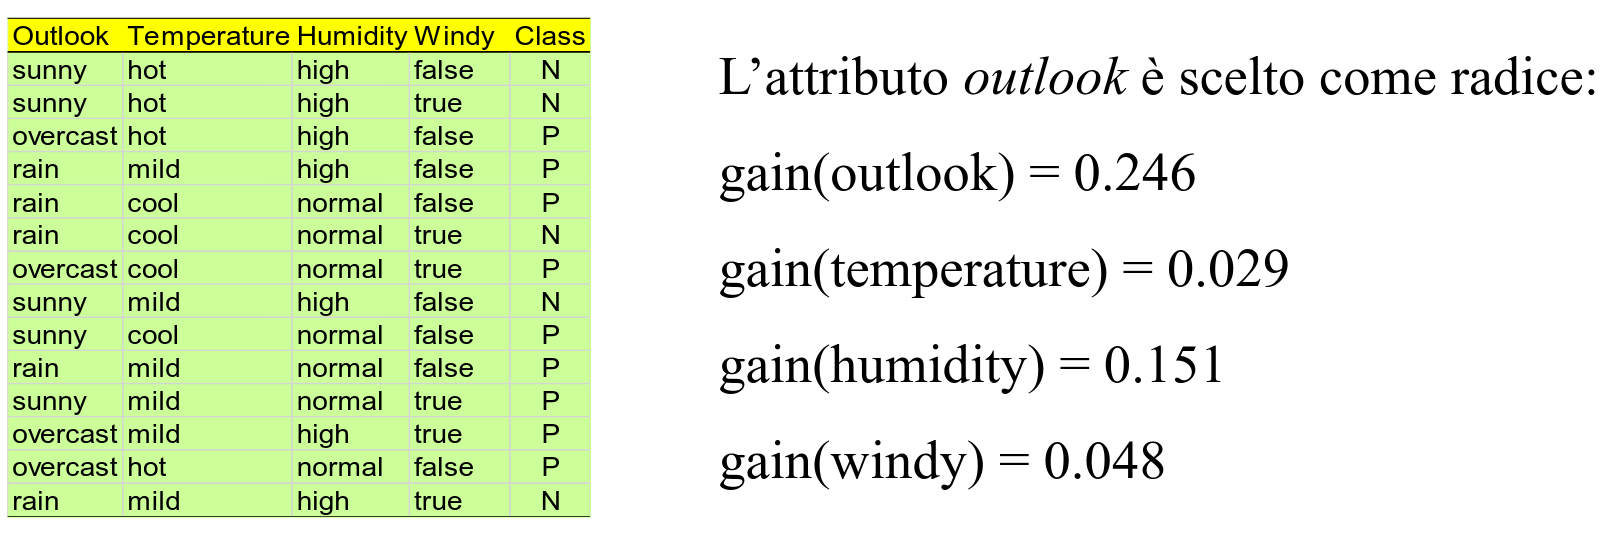
\includegraphics[width=.75\textwidth]{images/ig_outlook_example.png}
  \caption{Esempio di scelta della radice con Information Gain sul dataset “weather”.}
  \label{fig:ig-weather}
\end{figure}


\backmatter
% (eventuali appendici)
% \appendix
% \include{appendici}

% (eventuale bibliografia)
% \bibliographystyle{plain}
% \bibliography{bibliografia}

\end{document}
